\documentclass{article}



% Packages hyperref and algorithmic misbehave sometimes.  We can fix
% this with the following command.
%\newcommand{\theHalgorithm}{\arabic{algorithm}}

% Employ the following version of the ``usepackage'' statement for
% submitting the draft version of the paper for review.  This will set
% the note in the first column to ``Under review.  Do not distribute.''
\usepackage{icml2015} 
\usepackage{macros}
\usepackage{xr}
\externaldocument{appendix}


\begin{document}

\twocolumn[
\icmltitle{Cumulative Prospect Theory Meets Reinforcement Learning: Prediction and Control}

% It is OKAY to include author information, even for blind
% submissions: the style file will automatically remove it for you
% unless you've provided the [accepted] option to the icml2015
% package.
\icmlauthor{Your Name}{email@yourdomain.edu}
\icmladdress{Your Fantastic Institute,
            314159 Pi St., Palo Alto, CA 94306 USA}
\icmlauthor{Your CoAuthor's Name}{email@coauthordomain.edu}
\icmladdress{Their Fantastic Institute,
            27182 Exp St., Toronto, ON M6H 2T1 CANADA}

% You may provide any keywords that you 
% find helpful for describing your paper; these are used to populate 
% the "keywords" metadata in the PDF but will not be shown in the document
\icmlkeywords{boring formatting information, machine learning, ICML}

\vskip 0.3in
]

\begin{abstract}
Cumulative prospect theory (CPT) is known to model human decisions well, with substantial empirical evidence supporting this claim. 
CPT works by distorting probabilities and is more general than the classic expected utility and coherent risk measures. We bring this idea to a risk-sensitive reinforcement learning (RL) setting and design algorithms for both estimation and control.
The RL setting presents two particular challenges when CPT is applied: estimating the CPT objective requires estimations of the {\it entire distribution} of the value function and finding a {\it randomized} optimal policy.
The estimation scheme that we propose uses the empirical distribution to estimate the CPT-value of a random variable. We then use this scheme in the inner loop of policy optimization procedures for a stochastic shortest path problem. 
We propose a gradient-based policy optimization algorithmbased on the well-known simulation optimization idea of simultaneous perturbation stochastic approximation (SPSA).
We provide theoretical convergence guarantees for all the proposed algorithms and also empirically demonstrate the usefulness of our algorithms. 
\end{abstract}

% \keywords{
% Cumulative prospect theory, reinforcement learning, Service systems,  labor optimization, Adaptive labor staffing, Simultaneous
% perturbation stochastic approximation.
% }



\section{Introduction}
\label{sec:introduction}

Since the beginning of its history, mankind is deeply immersed in 
	designing and improving systems to serve humans needs.
Policy makers are busy with designing 
	systems that serve the education, transportation, economic, health and other 
	needs of the public,
while private sector enterprises or occupied at creating 
	and optimizing systems to serve other 
	specific needs of customers.
While it has been long recognized that 
	understanding human behavior is a prerequisite 
	to best serving the needs of humans \citet{},
%	and the private sector has adopted this strategy a while ago \citet{}
%	and the private sector quickly adopted this strategy,
	it is only recently that this approach is gaining a wider recognition.%
\footnote{
As evidence for this wider recognition in the public sector,
we can mention a recent executive order of the white house
calling for the use of behavioral science in public policy making, 
or the establishment of the ``Committee on Traveler Behavior and Values'' in the Transportation
Research Board in the US.}
%Using Behavioral Science Insights to Better Serve the American People

In this paper we consider \emph{human-centered reinforcement learning problems}
where the  reinforcement learning agent controls a system 
to produce long term outcomes (``return'') that are maximally aligned with the preferences of 
one or possibly multiple humans, an arrangement shown on Figure~\ref{fig:flow}.
As a running example, consider traffic optimization where the goal is to maximize
travelers' satisfaction, a problem many of us would agree is 
perhaps still inadequately addressed today, at least in many big cities.
In this example, the outcomes (``return'') are travel times, or delays. 
To capture human preferences, the outcomes are mapped to a single numerical quantity.
%We will make the assumption that human preferences can 
%To create a single numerical quantity that faithfully captures human preferences, 
%a \emph{risk metrics}, mapping the random returns to some scalar deterministic quantity, is used.
While preferences of rational agents facing uncertain situations can be modeled by expected utilities 
(i.e., the expectation of a nonlinear transformation, such as the exponential function of the rewards or costs) 
\citep{NeuMo44,fishburn1970expectedutility}, 
it is well known that
\todoc{Some use the world uncertainty in relation to situations
which can not be modeled probabilistically, and use risk in relation to situations that can be modeled probabilistically.
So we are inconsistent with these people.}
	humans are not rational in the mathematical sense
	but are subject to various emotional and cognitive biases.
As such, human preferences 
	are inconsistent with expected utilities, and in particular humans tend to have preferences 
	that cannot be modeled by using expected utilities alone
	 \citep{allais53,ellsberg61,kahneman1979prospect}.
An approach that gained 
%Behavioral scientists use alternate approaches to model human preferences.
	strong support amongst behavioral scientists and economists,  \citep[e.g.,][]{starmer2000developments,quiggin2012generalized},
	is based on \cite{kahneman1979prospect}'s celebrated \emph{prospect theory}.
In this work, we will use the so-called \emph{cumulative prospect theory} (CPT),
 	a refined variant of prospect theory due to \cite{tversky1992advances}, 
	which is even more supported than prospect theory.
CPT generalizes expected utility theory in that in addition to having a utility function transforming
	the outcomes, another function is introduced which distorts the probabilities in the cumulative distribution function.
As compared to prospect theory, CPT is monotone with respect to stochastic dominance, a property
	that is thought to be useful and often consistent with human preferences.	
	
\if0	

Popular approaches that use such risk metrics include the exponential utility formulation 
(cf. \cite{borkar2010learning}) that implicitly controls the variance.
An alternative is a to consider constrained formulations 
with explicit constraints on the variance of the return (cf. \cite{tamar2012policy,Prashanth13AC}). 
Another constraint alternative is to bound a coherent risk measure such as Conditional Value-at-Risk (CVaR), 
while minimizing the usual cost objective (cf. \cite{borkar2010risk,prashanth2014policy}).  

The risk metrics underlying the above-mentioned works 
are based on the assumption that human decision makers are rational and/or consistent.
While this may hold in certain restricted settings, a large body of literature indicates that humans are neither rational,
\todoc{Add literature supporting this. At least three books:)}
nor consistent (which, in fact, is an unsurprising fact, at least in the experience of the authors of the paper).
In other words, traditional approaches are based on the belief that optimizing the expected utility (EU) is appealing for human subjects. However, there is substantial evidence that this is not case - see 
the survey article \cite{starmer2000developments} and Chapter 4 of the book \cite{quiggin2012generalized}. In particular, the aforementioned references describe the Allais and Ellsberg paradoxes popular among economists for arguing against EU. 
Thus, if the goal is to produce outcomes that are best aligned with human preferences,
an alternative approach is required.
A singularly popular and successful approach in behavioral science and economics
is based on \textit{prospect theory (PT)} \cite{kahneman1979prospect} 
and its later enhancement, the so-called \textit{cumulative prospect theory} (CPT) \cite{tversky1992advances}.
CPT is a rank dependent expected utility model \cite{quiggin2012generalized} that incorporates decision weights to distort probabilities. 
The suitability of this approach to model human decision making (and thus preferences) has been widely documented \cite{prelec1998probability}, \cite{wu1996curvature}, \cite{conlisk1989three}, \cite{camerer1989experimental}, \cite{camerer1992recent}, \cite{harless1992predictions}, \cite{sopher1993test}, \cite{camerer1994violations}, \cite{gonzalez1999shape}, \cite{abdellaoui2000parameter}.
PT/CPT has been applied in a variety of domains, for e.g., healthcare \cite{lenert1999associations},  seismic design \cite{goda2008application}, transportation \cite{gao2010adaptive},\cite{fujii2004drivers}, \cite{ramming2001network}, online auctions \cite{weinberg2005exploring}, insurance  \cite{machina1995non} and finance \cite{barberis1999prospect}, \cite{epstein1989substitution}, \cite{epstein1991substitution}.
\fi

\tikzset{
  pobl/.style={
    inner sep=0pt, outer sep=0pt, fill=#1,
  },
  pobl gron/.style n args={2}{
    pobl=#1, rounded corners=#2,
  },
  pics/person/.style n args={3}{
    code={
      \node (-corff) [pobl=#1, minimum width=.25*#2, minimum height=.375*#2, rotate=#3, pic actions] {};
      \node (-pen) [minimum width=.3*#2, circle, pobl=#1, outer sep=.01*#2, anchor=south, rotate=#3, pic actions] at (-corff.north) {};
      \node (-coes dde) [pobl gron={#1}{1pt}, anchor=north west, minimum width=.12125*#2, minimum height=.25*#2, rotate=#3, pic actions] at (-corff.south west) {};
      \node [pobl=#1, anchor=north, minimum width=.12125*#2, minimum height=.15*#2, rotate=#3, pic actions] at (-coes dde.north) {};
      \node (-coes chwith) [pobl gron={#1}{1pt}, anchor=north east, minimum width=.12125*#2, minimum height=.25*#2, rotate=#3, pic actions] at (-corff.south east) {};
      \node [pobl=#1, anchor=north, minimum width=.12125*#2, minimum height=.15*#2, rotate=#3, pic actions] at (-coes chwith.north) {};
      \node (-braich dde) [pobl gron={#1}{.75pt}, minimum width=.075*#2, minimum height=.325*#2, outer sep=.0064*#2, anchor=north west, rotate=#3, pic actions] at (-corff.north east)  {};
      \node [pobl=#1, minimum width=.05*#2, minimum height=.2*#2, outer sep=.0064*#2, anchor=north west, rotate=#3, pic actions] at (-corff.north east) {};
      \node (-braich chwith) [pobl gron={#1}{.75pt}, minimum width=.075*#2, minimum height=.325*#2, outer sep=.0064*#2, anchor=north east, rotate=#3, pic actions] at (-corff.north west) {};
      \node [pobl=#1, minimum width=.0375*#2, minimum height=.2*#2, outer sep=.0064*#2, anchor=north east, rotate=#3, pic actions] at (-corff.north west) {};
      \node (-fit person) [fit={(-pen.north) (-braich dde.east) (-coes chwith.south) (-braich chwith.west)}] {};
      %\node (-pwy) [below=25pt of -fit person, every pin] {\tikzpictext};
      %\draw [every pin edge] (-fit person) -- (-pwy);
    },
  },
}
\tikzstyle{block} = [draw, fill=white, rectangle,
   minimum height=3em, minimum width=6em]
\tikzstyle{sum} = [draw, fill=white, circle, node distance=1cm]
\tikzstyle{input} = [coordinate]
\tikzstyle{output} = [coordinate]
\tikzstyle{pinstyle} = [pin edge={to-,thin,black}]

\begin{figure}[h]
\centering
\scalebox{0.5}{\begin{tikzpicture}
\node [block,fill=blue!20, minimum height=4em,] (world) {\makecell{\large\bf World}}; 
\node [block,fill=red!20, below=2.5cm of world] (agent) {\makecell{\large\bf Agent}}; 
\node [circle,fill=brown!50!black,right=2cm of world,label=above:{\bf Reward}] (tmp) {};
\coordinate [below left=2.5cm of world] (tmp2);
\coordinate [below right=1cm of agent] (belowagent);

\draw [->,thick] (world)  -| (tmp) |-   (agent);
\draw [->,thick] (agent)  -| (tmp2) |-   (world);
%\draw [->] (agent) --   (world);
\draw pic (person)  [right =3cm of tmp] {person={blue}{50pt}{0}};
\coordinate [right=2.8cm of tmp] (tmp3);
\coordinate [right=3.3cm of tmp] (tmp31);
\coordinate [right=1cm of tmp3] (belowhuman);
\coordinate [right=2.5cm of tmp3] (tmp4);
\draw [->,thick] (tmp) --   (tmp3);
\draw [-,thick,dotted] (tmp31)  -- node[below right=0.1cm and 0.5cm] {\textbf{CPT}} (belowhuman) --  (tmp4);
\draw [->,thick,dotted] (tmp4)  |-  (belowagent) -|  (agent.south);
\end{tikzpicture}}
\caption{Operational flow of a human-based decision making system
\todoc[inline]{Can we add next to the human a heart or something expressing that the human has feelings/preferences?
Alternatively, make an arrow that comes out from the human to the right, and write CPT on it.
}
}
\label{fig:flow}
\end{figure}
%\begin{tikzpicture}
  %[
    %every pin edge/.append style={latex-, shorten <=-2.5pt},
  %]

\if0
As illustrated in Figure \ref{fig:flow}, we consider a typical RL setting where the environment is unknown, but can be experimented with and propose a CPT based risk metric as the long-term performance objective.  \todoc{This para may need to be rewritten in light that I rewrote the previous one.}
\todoc{Risk measure is a technical term according to wikipedia. Risk metric does not seem to have this technical meaning so I propose using risk metric everywhere.}
CPT is a non-coherent and non-convex measure \todoc{I find it strange to emphasize only these aspects.
What's the goal of announcing these here?}
that is well known among psychologists and economists to be a good model for human decision-making systems, with strong empirical support.
To put it differently, CPT captures well the way humans evaluate outcomes and hence, we offer a CPT-variant of the RL notion of ``value function''. Unlike the regular value function which is the expectation of the return random variable, CPT-value employs a functional that distorts the underlying probabilities. The latter is achieved by fitting CPT model parameters to capture human preferences. The goal then for the learning system is to find a policy that maximizes the CPT-value of ``return''. 
\fi
%
%In the realm of sequential decision making under uncertainty, we propose a CPT-based risk measure.  In particular,  
%The current RL solutions cannot handle distortions and my current work is to develop both prediction and control schemes for probabilistically distorted MDPs.
%
%\todop[inline]{Add refs for distorted weights}
%In this paper, we consider a risk measure based on \textit{cumulative prospect theory} (CPT) \cite{tversky1992advances}, which is a non-coherent and non-convex measure that is well known among psychologists and economists to be a good model for human decision-making systems, with strong empirical support. In this paper, we incorporate CPT-based criteria into the classic objective \textit{value function} in a reinforcement learning framework. Intuitively this combination is appealing because it taps into the notion of how humans evaluate outcomes and also, a CPT objective leads to a randomized policy, which although harder to estimate often leads to more intuitively appealing behavior, as illustrated via an example below and also the numerical experiments later.

%%%%%%%%%%%%\
\paragraph{Our contributions:}
This is the first work to combine CPT with RL, and although on the surface it might seem straightforward, in fact there are many research challenges that arise from trying to apply a CPT objective in the RL framework. We outline these challenges as well as our solution approach below. \\
\textbf{\textit{Prediction:}} In the case of the classic value function, which is an expectation, a simple sample mean can be used for estimation, facilitating the use of temporal difference type algorithms. On the other hand, 
CPT-value   involves a distribution that is distorted using non-linear weight functions and hence, 
requires that the \textit{entire} distribution to be estimated.\\ 
\textit{Solution:} 
We propose a quantile based scheme for estimating the CPT-value.
We provide both asymptotic convergence and sample complexity results assuming the weight functions are either  \holder continuous, or
Lipschitz continuous, or
locally Lipschitz.
For the Lipschitz case, we obtain the canonical rate $O\left(\frac1{\epsilon^2}\right)$ for Monte Carlo-type schemes, while \holder continuous with constant $\alpha$ results in a rate  $O\left(\frac1{\epsilon^{2/\alpha}}\right)$, for achieving a $\epsilon$-close estimate.\\
\textbf{\textit{Control:}} 
Designing algorithms in order to find a \textit{CPT-optimal} policy is challenging because CPT-value is a non-coherent and non-convex risk measure that does not lend itself to dynamic programming approaches such as value/policy iteration due to the lack of a ``Bellman equation''. 
Thus, it is necessary to design new simulation optimization scheme that use sample CPT-value estimates to optimize the policy, which is generally \textit{randomized}. While classic simulation optimization settings usually have a zero mean noise in function evaluations, our setting one has to tradeoff simulation cost with the bias in a manner such that the resulting policy optimization scheme cancels the bias effect and converges. \\
\textit{Solution:} 
Using the well-known idea of simultaneous perturbation stochastic approximation (SPSA) from the \textit{simulation optimization} literature \cite{fu2015handbook}, we propose and analyze a gradient method for CPT value optimization in sequential decision making problems
under uncertainty.
Since SPSA by default assumes that the unbiased point-estimates of the optimization objective are available, which
is not the case in our problem, we extend the analysis of SPSA to handle the case when the optimization objective estimates are noisy, with controlled bias.
%
%We derive the condition that specifies the rate at which the number of samples for predicting the CPT-value should increase such that the bias of CPT-value estimates vanishes asymptotically (see (A3) later).
%
%, while the second is a Newton algorithm that also uses SPSA-based estimates of the gradient and also the Hessian. We remark again that, unlike traditional settings for SPSA, our estimates for CPT-value have a non-zero (albeit controlled) bias. We establish that our algorithms converge to a locally CPT-value optimal policy. 

To put things in context, risk-sensitive reinforcement learning problems are generally hard to solve. 
For a discounted MDP, \cite{Sobel82VD} showed that there exists a Bellman equation for the variance of the return, but the underlying Bellman operator is not necessarily monotone and this rules out policy iteration as a solution approach for variance-constrained MDPs.
Further, even if the transition dynamics are known, \cite{mannor2013algorithmic} show that finding a globally mean-variance optimal policy in a discounted MDP is NP-hard.
For average reward MDPs, \cite{filar1989variance} motivate a different notion of variance and then provide NP-hardness results for finding a globally variance-optimal policy.
CVaR as a risk measure is equally complicated as the measure here is a conditional expectation, where the conditioning is on a low probability event. Apart from the hardness of finding CVaR-optimal solutions, estimating CVaR for a fixed policy in a typical RL setting itself is a challenge considering CVaR relates to rare events and to the best of our knowledge, there is no algorithm with theoretical guarantees to estimate CVaR without wasting a lot of samples. There are proposals based on importance sampling (cf. \cite{prashanth2014policy,tamar2014optimizing}), but they lack theoretical guarantees. 

In contrast, we derive a \textit{provably} sample-efficient scheme for estimating the CPT-value (see next section for a precise definition) for a given policy and use this as the inner loop in a policy optimization scheme. Finally, we point out that the CPT-value that we define is a generalization in the sense that one can recover the regular value function and the risk measures such as VaR and CVaR by appropriate choices of a certain weight function used in the definition of CPT value.

\noindent
\textit{\textbf{Closest related work}} is \cite{lin2013stochastic}, where the authors propose a CPT-measure for an abstract MDP setting (see \cite{bertsekas2013abstract}). We differ from \cite{lin2013stochastic} in several ways:
\begin{inparaenum}[\bfseries (i)]
\item We do not have a nested structure for the CPT-value \eqref{eq:cpt-mdp} and this implies the lack of a Bellman equation for our CPT measure; and
\item We do not assume model information, i.e., we operate in a model-free RL setting. Moreover, we develop both estimation and control algorithms with convergence guarantees for the CPT-value function.
\end{inparaenum}

%The rest of the paper is organized as follows: 
%In Section~\ref{sec:cpt-val}, we introduce the notion of CPT-value of a general random variable $X$ and make a special case illustration when $X$ is the return of a stochastic shortest path problem.
%In Section~\ref{sec:cpt-sampling}, we
%describe the empirical distribution based scheme for estimating the CPT-value of any random variable. In Sections \ref{sec:1spsa}--\ref{sec:2spsa}, we present the gradient-based algorithms for optimizing the CPT-value. Next, in Section \ref{sec:mras}, we present a gradient-free model-based algorithm for CPT-value optimization in an MDP. We provide the proofs of convergence for all the proposed algorithms in Section~\ref{sec:convergence}.
%We present the results from numerical experiments for the CPT-value estimation scheme in Section~\ref{sec:expts} and finally, provide the concluding remarks in Section~\ref{sec:conclusions}.

%%%%%%%%%%%%%5
\section{CPT-value}
\label{sec:cpt-val}
For a real-valued random variable $X$, we first introduce a ``CPT-functional'' that replaces the traditional expectation. Subsequently, we specialize $X$ to be the return of stochastic shortest path problem.
\subsection{General definition}
The CPT-value of the random variable $X$ is a functional defined as
\begin{align}
\C_{u,w}(X) = &\intinfinity w^+(P(u^+(X)>z) dz\nonumber \\
& - \intinfinity w^-(P(u^-(X)>z) dz, \label{eq:cpt-general}
\end{align}
where $u=(u^+,u^-)$, $w=(w^+,w^-)$, $u^+,u^-:\R\rightarrow \R_+$ and $w^+,w^-:[0,1] \rightarrow [0,1]$ are continuous (see assumptions (A1)-(A2) in Section \ref{sec:cpt-sampling} for precise requirements on the $u$ and $w$). For notational convenience, we drop the dependence on $u,w$ and use $\C(X)$ to denote the CPT-value.  

Let us deconstruct the above definition:
 \begin{figure}[h]
   \centering
\tabl{c}{
%\includegraphics[width=3.8in]{utility.png}}
   \scalebox{0.5}{\begin{tikzpicture}
   \begin{axis}[width=13cm,height=6.5cm,legend pos=south east,
          %  grid = major,         
            axis lines=middle,
           % grid style={dashed, gray!30},
            xmin=-5,     % start the diagram at this x-coordinate
            xmax=5,    % end   the diagram at this x-coordinate
            ymin=-4,     % start the diagram at this y-coordinate
            ymax=4,   % end   the diagram at this y-coordinate
           % axis background/.style={fill=white},
            ylabel={\large\bf Utility},
            xlabel={\large\bf Gains},
            x label style={at={(axis cs:4.7,-0.8)}},
            y label style={at={(axis cs:-0.8,4.8)}},
            xticklabels=\empty,
            yticklabels=\empty
            ]
           \addplot[name path=cptplus,domain=0:5, green!35!black, very thick,smooth] 
              {pow(abs(x),0.8)}; 
            \addplot[name path=cptminus,domain=-5:0, red!35!black,very thick,smooth] 
              {-2*pow(abs(x),0.7)}; 
               \addplot[domain=-5:5, blue, thick]           {x}; 
               
               \path[name path=diagplus] (axis cs:0,0) -- (axis cs:5,5);
 			  \path[name path=diagminus] (axis cs:-5,-5) -- (axis cs:0,0);
                \path[name path=xaxisplus] (axis cs:0,0) -- (axis cs:5,0);
                 \path[name path=xaxisminus] (axis cs:-5,0) -- (axis cs:0,0);
                 \path[name path=yaxisplus] (axis cs:0,0) -- (axis cs:0,5);
                 \path[name path=yaxisminus] (axis cs:0,-5) -- (axis cs:0,0);
 
 \addplot [orange!40]  fill between[of= diagminus and yaxisminus];
 \addplot [cyan!20]  fill between[of= diagplus and xaxisplus];
 
 \node at (axis cs:  -3.7,-0.45) {\large\bf Losses};
 \node at (axis cs:  4,2.5) {\large $\bm{u^+}$};
 \node at (axis cs:  -1,-3) {\large $\bm{-u^-}$};
 \node at (axis cs:  2.5,-2.5) {\large\bf Baseline};
\draw[-{>[scale=2.5,
          length=5,
          width=3]},thick] (axis cs:2,-2) -- (axis cs:0,0);
   \end{axis}
   \end{tikzpicture}}}\\[1ex]
\caption{Utility function}
\label{fig:u}
\end{figure}

\paragraph{Utility functions:} $u^+, u^-$ are utility functions corresponding to gains ($X \ge 0$) and losses ($X \le 0$), respectively. For example, consider a scenario where one can either earn \$$500$ w.p $1$ or earn \$$1000$ w.p. $0.5$ (and nothing otherwise). The human tendency is to choose the former option of a certain gain. If we flip the situation, i.e., a certain loss of \$$500$ or a loss of \$$1000$ w.p. $0.5$, then humans choose the latter option.  Handling losses and gains separately is a salient feature of CPT, and this addresses the tendency of humans to play safe with gains and take risks with losses - see Fig \ref{fig:u}.  In contrast, the traditional value function makes no such distinction between gains and losses.  

\begin{figure}[h]
\centering
\tabl{c}{
%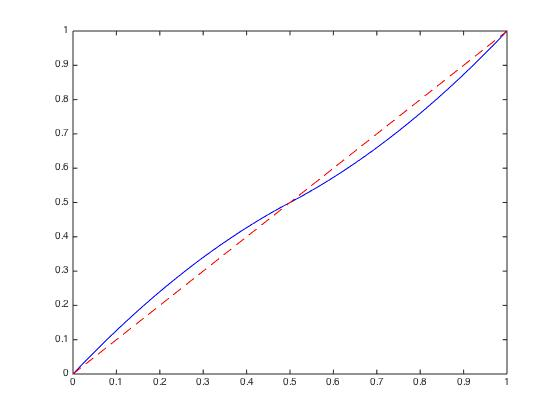
\includegraphics[width=8cm]{results/Probability_weighting_function.jpg}
  \scalebox{0.65}{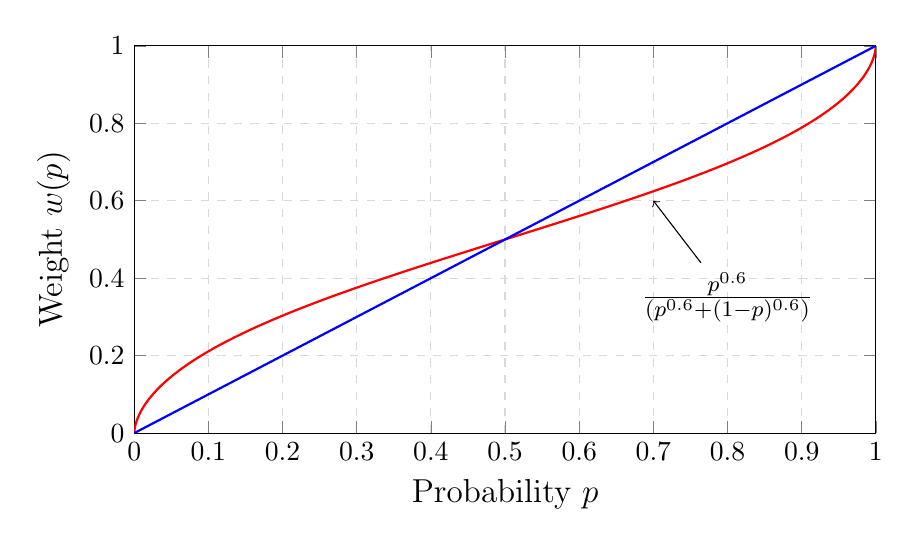
\begin{tikzpicture}
  \begin{axis}[width=11cm,height=6.5cm,legend pos=south east,
           grid = major,
           grid style={dashed, gray!30},
           xmin=0,     % start the diagram at this x-coordinate
           xmax=1,    % end   the diagram at this x-coordinate
           ymin=0,     % start the diagram at this y-coordinate
           ymax=1,   % end   the diagram at this y-coordinate
           axis background/.style={fill=white},
           ylabel={\large Weight $\bm{w(p)}$},
           xlabel={\large Probability $\bm{p}$}
           ]
          \addplot[domain=0:1, red, thick,smooth,samples=1500] 
             {pow(x,0.6)/(pow(x,0.6) + pow(1-x,0.6))}; 
             \node at (axis cs:  0.8,0.35) (a1) {\large $\bm{\frac{p^{0.6}}{(p^{0.6}+ (1-p)^{0.6})}}$};           
             \draw[->] (a1) -- (axis cs:  0.7,0.6);
                 \addplot[domain=0:1, blue, thick]           {x};                      
  \end{axis}
  \end{tikzpicture}}\\[1ex]
}
\caption{Weight function}
\label{fig:w}
\end{figure}

\paragraph{Weight functions:} $w^+, w^-$ are functions corresponding to gains and losses, respectively. 
The main idea is that humans deflate high-probabilities and inflate low-probabilities and this is the rationale behind using a weight function in CPT.
For example, humans usually choose a stock that gives one million dollars w.p. $1/10^6$ over one that gives \$$1$ w.p. $1$ and the reverse when signs are flipped. 
Thus the value seen by the human subject is non-linear in the underlying probabilities - an observation with strong empirical evidence that used human subjects \citep{tversky1992advances}.  In contrast,the traditional value function is linear in the underlying probabilities. 
As illustrated with $w=w^+=w^-$ in Fig \ref{fig:w}, the weight functions are continuous, non-decreasing and  have the range $[0,1]$ with $w^+(0)=w^-(0)=0$ and $w^+(1)=w^-(1)=1$. 
The authors in \cite{tversky1992advances} recommend $w(p) = \frac{p^{\delta}}{{(p^{\delta}+ (1-p)^{\delta})}^{1/\delta}}$, while \cite{prelec1998probability} recommends $w(p) = \exp(-(-\ln p)^\delta)$, with $0 < \delta <1$ and in both cases, the weight function has the inverted-s shape, which is seen to be a good fit from empirical tests on human subjects - see \cite{conlisk1989three}, \cite{camerer1989experimental}, \cite{camerer1992recent}, \cite{harless1992predictions}, \cite{sopher1993test}, \cite{camerer1994violations}, \cite{gonzalez1999shape}, \cite{abdellaoui2000parameter}.  
Weight functions can explain non-linear probability distortions, as illustrated by the following example: \\
\textit{\textbf{[Stock 1]}} This investment results in a gain of \$$10$ with probability (w.p.) $0.1$ and a loss of \$$500$ w.p. $0.9$. The expected return is \$$-449$, but this does not necessarily imply that ``human'' investors' evaluation of the stock is \$$-449$. Instead, it is very likely that the humans evaluate it to a higher value, e.g. \$$-398$ ($=$ gain w.p. $0.2$ and loss w.p. $0.8$).\footnote{See Table 3 in \cite{tversky1992advances} to know why such a human evaluation is likely.}\\
\textit{\textbf{[Stock 2]}} loss of \$$10$ w.p. $0.9$, gain \$$500$ w.p. $0.1$. Expected return: \$$41$; Human evaluation: \$$92$ ($=$ loss w.p. $0.8$).\\
\textit{\textbf{[Stock 3]}} loss of \$$10$ w.p. 0.1, gain \$$500$ w.p. $0.9$. Expected return: \$$449$; Human evaluation: \$$398$ ($=$ loss w.p. $0.2$). 


\paragraph{Optimization objective:} Suppose the r.v. $X$ is a function of a $d$-dimensional parameter $\theta$. The goal then is to solve the following problem:
\begin{align}
\label{eq:opt-general}
\textrm{Find ~}\theta^* = \argmax_{\theta \in \Theta} \C(X^\theta),
\end{align}
where $\Theta$ is a compact and convex subset of $\R^d$.
The above optimization problem has several applications in RL. For instance, $X$ could be the total reward/discounted reward/average reward r.v. for a fixed policy (given as $\theta$) in the context of a stochastic shortest path/discounted/average reward MDP, respectively. We illustrate one of these applications next.

\subsection{Application: Stochastic Shortest Path}
We consider a stochastic shortest path (SSP) problem with states $\S=\{0,\ldots,\L\}$, where $0$ is a special reward-free absorbing state.  A randomized policy $\pi$ is a function that maps any state $s\in \S$ onto a probability distribution over the actions $\A(s)$ in state $s$. As is standard in policy gradient algorithms, we parameterize $\pi$ and assume it is continuously differentiable in its parameter $\theta \in \R^d$.  
An \textit{episode} is a simulated sample path using policy $\theta$ that starts in state $x^0\in \S$, visits $\{x_1,\ldots, x_{\tau-1}\}$ before ending in the absorbing state $0$, where $\tau$ is the first passage time to state $0$.
Let $D^\theta(x^0)$ be a random variable (r.v) that denote the total reward from an episode, defined by
$$ D^\theta(s^0) = \sum\limits_{m=0}^{\tau-1} r(s_m,a_m), $$
where the actions $a_m$ are chosen using policy $\theta$ and $r(s_m, a_m)$ is the single-stage reward in state $s_m\in \S$ when action $a_m \in \A(s_m)$ is chosen. 

Instead of the traditional RL objective for an SSP is to maximize the expected value $\E (D^\theta(x^0))$, 
we adopt the CPT approach and aim to solve the following problem: 
$$ \max_{\theta \in \Theta} \C(D^\theta(s^0)),$$
where $\Theta$ is the set of admissible policies that are \textit{proper}\footnote{A policy $\theta$ is proper if $0$ is recurrent and all other states are transient for the Markov chain underlying $\theta$. It is standard to assume that policies are proper in an SSP setting - cf. \cite{bertsekas1995dynamic}.} and the CPT-value function $\C(D^\theta(s^0))$ is defined as
\begin{align}
\C(D^\theta(s^0))& = \intinfinity w^+(P(u^+(D^\theta(s^0)))>z) dz \nonumber
\\&- \intinfinity w^-(P(u^-(D^\theta(s^0)))>z) dz. \label{eq:cpt-mdp}
\end{align}

\paragraph{Generalization:} It is easy to see that the CPT-value is a generalization of the traditional value function, as a choice of identity map for the weight and utility functions in \eqref{eq:cpt-mdp} makes it the expectation of the total cost $D^\theta)$.  It is also possible to get \eqref{eq:cpt-mdp} to coincide with coherent risk measures (e.g. CVaR) by the appropriate choice of weight functions.

\paragraph{Sensitivity:}
Traditional EU based approaches are sensitive to modeling errors as illustrated in the following example: 
Suppose stock $\cal{A}$ gains \$$10000$ w.p $0.001$ and loses nothing w.p. $0.999$, while stock $\cal B$ surely gains $11$. With the classic value function objective, it is optimal to invest in stock $\cal B$ as it returns $11$,  while $\cal A$ returns $10$ in expectation (assuming utility function to be the identity map). Now, if the gain probability for stock $\cal A$ was $0.002$, then it is no longer optimal to invest in stock $\cal B$ and investing in stock $A$ is optimal.
Notice that a very slight change in the underlying probabilities resulted in a big difference in the investment strategy and a similar observation carries over to a multi-stage scenario (see the house buying example in the numerical experiments section). 
 %A randomized policy that $50$\% in stock $\cal A$ and the rest in a risk-free asset is less sensitive to the error in under-estimating the loss probability. 

Using CPT makes sense because it inflates low probabilities and thus can account for modeling errors, especially considering that model information is unavailable in practice.
Note also that in MDPs with expected utility objective, there exists a deterministic policy that is optimal. However, with CPT-value objective, the optimal policy is \textit{not necessarily} deterministic - See also the organ transplant example on pp. 75-81 of \cite{lin2013stochastic}. 



%%%%%%%%%%%%%%%%%%%%%%%%%%%%%%%%%%%%%%%%%%%%%%%%%%%%%%%%%%%%%%
%%%%%%%%%%%%%%%%%%%%%%%%%%%%%%%%%%%%%%%%%%%%%%%%%%%%%%%%%%%%%%
%%%%%%%%%%%%%%%%%%%%%%%%%%%%%%%%%%%%%%%%%%%%%%%%%%%%%%%%%%%%%%
%%%%%%%%%%%%%%%%%%%%%%%%%%%%%%%%%%%%%%%%%%%%%%%%%%%%%%%%%%%%%%
%%%%%%%%%%%%%%%%%%%%%%%%%%%%%%%%%%%%%%%%%%%%%%%%%%%%%%%%%%%%%%
%%%%%%%%%%%%%%%%%%%%%%%%%%%%%%%%%%%%%%%%%%%%%%%%%%%%%%%%%%%%%%
%%%%%%%%%%%%%%%%%%%%%%%%%%%%%%%%%%%%%%%%%%%%%%%%%%%%%%%%%%%%%%
%%%%%%%%%%%%%%%%%%%%%%%%%%%%%%%%%%%%%%%%%%%%%%%%%%%%%%%%%%%%%%

\section{CPT-value estimation} 
\label{sec:cpt-sampling}

For the sake of notational simplicity, we let $X$ denote the r.v. $X^\theta$, i.e., where the parameter $\theta$ is assumed to be fixed for the purpose of CPT-value estimation in this section. 

\paragraph{On integrability}
Observe that the first integral in \eqref{eq:cpt-mdp}, i.e., 
\begin{align}
\label{eq:1st-int-cpt}
\int_0^{+\infty} w^+(P(u^+(X)>z)) d z
\end{align}
may diverge even if the first moment of random variable $u^+(X)$ is finite. 
For example, suppose $U$ has the tail distribution function
$$P(U>z)  = \frac{1}{z^2}, z\in [1, +\infty),$$
and $w^+(z)$ takes the form $w(z) = z^{\frac{1}{3}}$. Then, the integral \eqref{eq:1st-int-cpt} with respect to the distorted tail, i.e.,
$$
\int_1^{+\infty} \frac{1}{z^{\frac{2}{3}}} dz
$$
does not even exist. A similar argument applies to the second integral in \eqref{eq:cpt-mdp} as well.

To overcome the above integrability issues, we make different assumptions on the weight and/or utility functions. In particular, we assume that the weight functions $w^+, w^-$ are either 
\begin{inparaenum}[\bfseries (i)]
\item Lipschitz continuous, or
\item \holder continuous, or
\item locally Lipschitz.
\end{inparaenum}
We devise a scheme for estimating \eqref{eq:cpt-mdp} given only samples from $X$ and show that, under each of the aforementioned assumptions, our estimator (presented next) converges almost surely. 
We also provide sample complexity bounds assuming that the utility functions are bounded.

% \subsubsection*{Main results}
% As mentioned earlier, to overcome integrability issues, we make the following assumption:\\[1ex]
% \textbf{Assumption (A1).}  The weight functions $w^+, w^-$ are Lipschitz with common constant $L$, and 
% $u^+(X)$ and $u^-(X)$ both have bounded first moments\\[1ex]
% % If the weight function is not Lipschitz, then the integrals using the distribution of $X$ in CPT-value may not even be finite. 
% We make the following assumptions on the utility functions:\\[1ex]
% \textbf{Assumption (A2).}  The utility functions $u^+(X)$ and $u^-(X)$ are continuous and increasing.\\[1ex]
% \todoj{Check if increasing is necessary}
% \textbf{Assumption (A2').}  In addition to (A2), the utility functions $u^+(X)$ and $u^-(X)$ are bounded above by $M<\infty$.\\[1ex]
% For the convergence rate results below, we require (A2'), while (A2) is sufficient to prove asymptotic convergence.
% 
% The following result shows that the estimate \eqref{eq:cpt-est} converges to the true CPT value almost surely and at the (nearly) canonical Monte Carlo asymptotic rate. 
% \begin{proposition} (\textbf{Asymptotic convergence and rate.})
% \label{thm:asymp-conv}
% Under (A1) and (A2), we have
% \begin{align}
% \widehat V_n(X) \rightarrow \C(X) \text{ a.s. as } n \rightarrow \infty.
% \end{align}
% If we assume (A2'), then we have
% $$
% \limsup_{n\rightarrow \infty} \sqrt{\frac{n}{2 \ln \ln n}} ||\hat{V_n}(X)-\C(X)||_{\infty} 
% \leq  LM \quad \text{a.s.}
% $$
% \end{proposition}
% \begin{proof}
%  See Section \ref{appendix:cpt-est}.
% \end{proof}
% 
% While the above result establishes that \eqref{eq:cpt-est} is an unbiased estimate in the asymptotic sense, it is important to know the rate at which the estimate in \eqref{eq:cpt-est} converges to the CPT-value. 
% The following sample complexity result shows that $O\left(\frac{1}{\epsilon^2}\right)$ number of samples are required to be $\epsilon$-close to the CPT-value in high probability.
% \begin{proposition}(\textbf{Sample Complexity})
% \label{thm:dkw}
% Under (A1) and (A2'), for any $\epsilon, \delta >0$, we have
% \begin{align*}
% P(|\widehat V_n(X) - \C(X)|\le\epsilon) \geq  1 - \delta, \,\,\, \forall n \geq \frac{2 L^2 M^2}{\epsilon^2} ln \frac{4}{\delta}.
% \end{align*}
% \end{proposition}
% \begin{proof}
%  See Section \ref{appendix:cpt-est}.
% \end{proof}

%%%%%%%%%%%%%%%%%%%%%%%%%%%%%%%%%%%%%%%%%%%%%%%%%%%%%%%%%%%%%%
%%%%%%%%%%%%%%%%%%%%%%%%%%%%%%%%%%%%%%%%%%%%%%%%%%%%%%%%%%%%%%
\subsection{Estimation scheme for \holder continuous weights}
Recall the H\"{o}lder continuity property first in definition 1:
\begin{definition}
{\textbf{\textit{(H\"{o}lder continuity)}}}
If $0 < \alpha \leq 1$, a function $f \in C([a,b])$ is said to satisfy
a H\"{o}lder condition of order $\alpha$ (or to be H\"{o}lder continuous
of order $\alpha$) if
\[
\sup_{x \neq y} \frac{| f(x) - f(y) |}{| x-y |^{\alpha}} \leq C .
\]
\end{definition}

In order to ensure integrability of the CPT-value \eqref{eq:cpt-mdp}, we make the following assumption:\\[1ex]
\textbf{Assumption (A1).}  
The weight functions $w^+, w^-$ are H\"{o}lder continuous with common order $\alpha$. Further,
$\exists \gamma \le \alpha \text{   s.t,  }$ 
$$\int_0^{+\infty} P^{\gamma} (u^+(X)>z) dz < +\infty \text{ and }\int_0^{+\infty} P^{\gamma} (u^-(X)>z) dz < +\infty$$

The above assumption ensures that the CPT-value as defined by \eqref{eq:cpt-mdp} is finite - see Proposition \ref{prop:Holder-cpt-finite} in Section \ref{sec:holder-proofs} for a formal proof.


\paragraph{Approximating CPT-value using quantiles:}
Let $\xi^+_{\frac{i}{n}}$ denote the $\frac{i}{n}$th quantile of the r.v. $u^+(X)$. Then, it can be seen that (see Proposition \ref{prop:holder-quantile} in Section \ref{sec:holder-proofs})
\begin{align}
\label{eq:holder-quant-motiv}
\lim_{n \rightarrow \infty} \sum_0^{n-1} \xi^+_{\frac{i}{n}} \left(w^+\left(\frac{n-i}{n}\right)- w^+\left(\frac{n-i-1}{n}\right) \right) = \int_0^{+\infty} w^+(P(u^+(X)>z)) dz.
\end{align}

The identical property holds for the pairs $u^-(X)$, $\xi^-_{\frac{i}{n}}, w^-$ , with $\xi^-_{\frac{i}{n}}$ denote the 
$\frac{i}{n}$th quantile of the r.v. $u^-(X)$.

However, we do not know the distribution of $u^+(X)$ or $u^-(X)$ and hence, we develop a procedure that uses order statistics for estimating quantiles, which in turn assists in estimating the CPT-value along the lines of \eqref{eq:holder-quant-motiv}. The estimation scheme is presented in Algorithm \ref{alg:holder-est}.

\todoj[inline]{Need some text here to connect the quantile business to EDFs, i.e., to say that step 5 in Algo 1 is the same as estimating EDFs and then doing empirical integration using EDFs to estiamete CPT-value}

\begin{algorithm}
\caption{CPT-value estimation for \holder continuous weights}
\label{alg:holder-est}
\begin{algorithmic}[1]
\State Simulate $n$ random samples with distribution $X$, sort them and denoted the ordered sample as 
$X_{[1]}, X_{[2]}, \ldots X_{[n]}$.
\State Calculate $u^+(X_{[1]}),\ldots u^+(X_{[n]})$
\State Order the simulated samples and label them as follows: 
$u^+(X_{[1]}),\ldots,u^+(X_{[n]})$.
\State Use $u^+(X_{[i]}), i\in \mathbb{N}\cap (0,n)$ as an approximation for the $\frac{i}{n} th$ quantile of $u^+(X)$, i.e, $\xi_{\frac{i}{n}}, i\in \mathbb{N}\cap (0,n)$.
\State Denote the statistic 
$\overline \C_n^+:=\sum_{i=1}^{n-1} u^+(X_{[i]}) (w^+(\frac{n-i}{n})- w^+(\frac{n-i-1}{n}) )$
\State Repeat the procedure on the sequence $X_{[1]}, X_{[2]}, \ldots X_{[n]}$, with respect to the function $u^-$, 
and denote the statistic $\overline \C_n^-:=\sum_{i=1}^{n-1} u^-(X_{[i]}) (w^-(\frac{n-i}{n})- w^-(\frac{n-i-1}{n}) ) $
\State Return the statistic $\overline \C_n =\overline \C_n^+ - \overline \C_n^-$.
\end{algorithmic}
\end{algorithm}

\subsubsection*{Main results}
We make the following assumptions on the utility functions:\\[1ex]
\textbf{Assumption (A2).}  The utility functions $u^+(X)$ and $u^-(X)$ are continuous and increasing.\\[1ex]
\todoj{Check if increasing is necessary}
\textbf{Assumption (A2').}  In addition to (A2), the utility functions $u^+(X)$ and $u^-(X)$ are bounded above by $M<\infty$.\\[1ex]
For the convergence rate results below, we require (A2'), while (A2) is sufficient to prove asymptotic convergence.

\begin{proposition}(\textbf{Asymptotic convergence.})
\label{prop:holder-asymptotic}
Assume (A1) and also that $F^+(\cdot)$,$F^-(\cdot)$ - the distribution functions of $u^+(X)$, and $u^-(X)$ are Lipschitz continuous with constants $L^+$ and $L^-$, respectively on the interval $(0,+\infty)$, and 
$(-\infty, 0)$ . Then, we have that
\begin{align}
\lim_{n\rightarrow +\infty} 
\overline \C_n
=
\C(X)
 \text{   a.s.,}
\end{align}
where $\overline \C_n$ is as defined in Algorithm \ref{alg:holder-est} and $\C(X)$ as in \eqref{eq:cpt-general}.
\end{proposition}
\begin{proof}
See Section \ref{sec:holder-proofs}.
\end{proof}

While the above result establishes that $\overline \C_n$ is an unbiased estimate in the asymptotic sense, it is important to know the rate at which the estimate $\overline \C_n$ converges to the CPT-value $\C(X)$. 
The following sample complexity result shows that $O\left(\frac{1}{\epsilon^{2/\alpha}}\right)$ number of samples are required to be $\epsilon$-close to the CPT-value in high probability.

% 
% While the above proposition gives an asymptotic guarantee, in the following we provide a sample complexity result for Algorithm \ref{alg:holder-est}.
% For this result, we assume, as in the case of Lipschitz continuous weights, that the utility functions are bounded in addition to (A1').

\begin{proposition}(\textbf{Sample complexity.})
\label{prop:holder-dkw}
Assume (A1) and (A2'). Then, $\forall \epsilon, \delta$, we have
$$
P(\left |\overline \C_n- \C(X) \right| \leq  \epsilon ) > \delta\text{     ,} \forall n \geq \ln(\frac{1}{\delta})\cdot 
\frac{4L^2 M^2}{\epsilon^{2/\alpha}}.$$
\end{proposition}
\begin{proof}
Notice the the following equivalence:
$$\sum_{i=1}^{n-1} u^+(X_{[i]}) (w^+(\frac{n-i}{n}) - w^+(\frac{n-i-1}{n})) =  \int_0^M w^+(1-\hat{F^+_n}(x)) dx, $$
and also,
$$\sum_{i=1}^{n-1} u^-(X_{[i]}) (w^-(\frac{n-i}{n}) - w^-(\frac{n-i-1}{n})) =  \int_0^M w^-(1-\hat{F^-_n}(x)) dx, $$

where $\hat{F^+_n}(x)$ and $\hat{F^-_n}(x)$ is the empirical distribution of $u^+(X)$
and $u^-(X)$, defined as follows:
\begin{align}
{\hat F_n}^+(x)=&\frac{1}{n} \sum_{i=1}^n 1_{(u^+(X_i) \leq x)}, 
{\hat F_n}^-(x)=\frac{1}{n} \sum_{i=1}^n 1_{(u^-(X_i) \leq x)}.
\label{eq:edf}
\end{align}

The main claim follows from the equivalence mentioned above together with the well-known DKW inequality.
The detailed proof is available in Section \ref{sec:holder-proofs}.
\end{proof}

\subsubsection*{Special case: Lipschitz continuous weights}
\textbf{Assumption (A1').}  The weight functions $w^+, w^-$ are Lipschitz with common constant $L$, and 
$u^+(X)$ and $u^-(X)$ both have bounded first moments.\\[1ex]

\begin{corollary}[Lipschitz case]
Assume (A1') and (A2). Then, we have that 
$$\lim_{n\rightarrow +\infty} \overline \C_n = \C(X) \text{   a.s.}$$

In addition, if we assume (A2'), we have 
$$
P(\left |\overline \C_n- \C(X) \right| \leq  \epsilon ) > \delta\text{     ,} \forall n \geq \ln(\frac{1}{\delta})\cdot 
\frac{4L^2 M^2}{\epsilon^{2}}.
$$
\end{corollary}
\begin{proof}
 Setting $\alpha=\gamma=1$ in the proof of Proposition \ref{prop:Holder-cpt-finite}, it is easy to see that the CPT-value \eqref{eq:cpt-mdp} is finite. Thus, the claims regarding asymptotic convergence and sample complexity as special cases of Proposition \ref{prop:holder-asymptotic}--\ref{prop:holder-dkw}, with $\alpha=1$. 
\end{proof}



%%%%%%%%%%%%%%%%%%%%%%%%%%%%%%%%%%%%%%%%%%%%%%%%%%%%%%%%%%%%%%
%%%%%%%%%%%%%%%%%%%%%%%%%%%%%%%%%%%%%%%%%%%%%%%%%%%%%%%%%%%%%%
%%%%%%%%%%%%%%%%%%%%%%%%%%%%%%%%%%%%%%%%%%%%%%%%%%%%%%%%%%%%%%
\subsection{Estimation scheme for locally Lipschitz weights and discrete $X$}
\todop[inline]{Would be better if the background been put to the introduction part}
<<<<<<< HEAD
\paragraph{Background.}
Here we assume that the r.v. $X$ is discrete valued.
Let $p_i, i=1,\ldots,K$ denote the probability of incurring a gain/loss $x_i, i=1,\ldots,K$. %Assume $x_1 \le \ldots \le x_K$. 
Given a utility function $u$ and weighting function $w$, \textit{\textbf{Prospect theory}} (PT) value is defined as $V(X) = \sum_{i=1}^K u(x_i) w(p_i)$. 
As explained in the introduction, the idea is to take an utility function that is $S$-shaped, so that it satisfies the \textit{diminishing sensitivity}  property. 
If we take the weighting function $w$ to be the identity, then one recovers the classic expected utility. A general weight function inflates low probabilities and deflates high probabilities and this has been shown to be close to the way humans make decisions (see \cite{kahneman1979prospect}, \cite{fennema1997original} for a justification, in particular via empirical tests using human subjects).
However, PT is lacking in some theoretical aspects as it violates first-order \textit{stochastic dominance}.\footnote{Consider the following example from \cite{fennema1997original}: Suppose there are $20$ prospects (outcomes) ranging from $-10$ to $180$, each with probability $0.05$. If the weight function is such that $w(0.05) > 0.05$, then it uniformly overweights all \textit{low-probability} prospects and the resulting PT value is higher than the expected value $85$. This violates stochastic dominance, since a shift in the probability mass from bad outcomes did not result in a better prospect.}

CPT uses a similar measure as PT, except that the weights are a function of cumulative probabilities. First, separate the gains and losses as 
$x_1\le \ldots \le x_l \le 0 \le x_{l+1} \le \ldots \le x_K$. Then, the CPT-value is defined as 
\begin{align}
\label{eq:cpt-discrete}
V(X) = &(u^-(x_1))\cdot w^-(p_1) 
+\sum_{i=2}^l u^-(x_i) \Big(w^-(\sum_{j=1}^i p_j) - w^-(\sum_{j=1}^{i-1} p_j)\Big) 
\\&
 + \sum_{i=l+1}^{K-1} u^+(x_i) \Big(w^+(\sum_{j=i}^K p_j) - w^-(\sum_{j=i+1}^K p_j) \Big)
 + u^+(x_K)\cdot w^+(p_K), 
\end{align} 
where $u^+, u^-$ are utility functions and $w^+, w^-$ are weight functions corresponding to gains and losses, respectively. The utility functions $u^+$ and $u^-$ are non-decreasing, while the weight functions are continuous, non-decreasing and have the range $[0,1]$ with $w^+(0)=w^-(0)=0$ and $w^+(1)=w^-(1)=1$ . 
Unlike PT, the CPT-value does not violate stochastic dominance.\footnote{In the aforementioned example, increasing $w^-(0.05)$ and $w^+(0.05)$ does not impact outcomes other than those on the extreme, i.e., $-10$ and $180$, respectively. For instance, the weight for outcome $100$ would be $w^+(0.45) - w^+(0.40)$. Thus, CPT formalizes the intuitive notion that humans are sensitive to extreme outcomes and relatively insensitive to intermediate ones.}

\paragraph{Estimation scheme.} 
Let $\hat{p_k}= \frac{1}{n} \sum_{i=1}^n I_{\{U =x_k\}}$. Then, we estimate $V(X)$ as follows:
\begin{align}
 \label{eq:cpt-discrete-est}
\hat V_n(X) = 
u^-(x_1)\cdot w^-(\hat p_1)+
& \sum_{i=2}^l u^-(x_i) \Big(w^-(\sum_{j=1}^i \hat p_j) - w^-(\sum_{j=1}^{i-1} \hat p_j)\Big) 
\\
&
+ \sum_{i=l+1}^{K-1} u^+(x_i) \Big(w^+(\sum_{j=i}^K \hat p_j) - w^-(\sum_{j=i+1}^K \hat p_j) \Big)+ u^+(x_K)\cdot w^+(\hat p_K).
\end{align}
Owing to the fact that $\hat{p_k}$ converge a.e to $p_k=P(X_i=x_k)$, with $X_i$ be the sample of $X$ the above estimator obtains strong consistency property according to continuous mapping theorem. 

\paragraph{Sample Complexity}
Before exploring on the convergence speed to the sample estimator, it is necessary to introduce Hoeffding's inequality:
\begin{lemma}
Let $Y_1,...Y_n$ be \emph{independent random variables} satisfying $P(a\leq Y_i \leq b)= 1,$ each i, where $a<b.
$Then for $t>0$,
$$P(\left|\sum_{i=1}^n Y_i -\sum_{i=1}^n E(Y_i)\right| \geq nt ) \leq 2\exp{\{-2nt^2 /(b-a)^2\}} $$
\end{lemma}

\noindent \textbf{Notations:} We will introduce 
\[
F_k = 
\begin{cases}
   \sum_{i=1}^k p_k & \text{if   } k \leq l \\
   \sum_{i=k}^K p_k & \text{if  }  k > l
\end{cases}  
\]

and $\hat F_k$ retains the same form as $F_k$ by replacing $p_k$ by $\hat p_k$ 
\\

\noindent The Hoeffding inequality suggests the following proposition:
\begin{proposition}
Let $F_k$ and $\hat F_k$ as introduced above, Then for every $\epsilon >0$, 
$$P(|\hat{F_k}-F_k| > \epsilon) \leq 2 e^{-2n \epsilon^2} $$
\end{proposition}
\begin{proof}
We focus on the case when $k > l$,and the case of $k \leq l$ will be proved through the same fashion.
Notice that when $k>l$,  $\hat F_k =I_{(U_i \geq  x_k) }$ and the random variables are independent to each other for each i, and it is bounded by 1. 
The probability $P(\left|F_k- F_k \right| > \epsilon)$ is equal to 
\begin{align*}
&
P(\left|\hat{F_k}- F_k \right| > \epsilon) \\ & = P(\left| \frac{1}{n} \sum_{i=1}^n I_{\{U_i \geq
x_k\}} - \frac{1}{n} \sum_{i=1}^n E(I_{\{U_i \geq x_k\}}) \right| > \epsilon) \\ & = P(\left|
\sum_{i=1}^n I_{\{U_i \geq x_k\}} - \sum_{i=1}^n E(I_{\{U_i \geq x_k\}}) \right| > n\epsilon) \\ &
    \leq 2e^{-2n \epsilon^2}
\end{align*}

\end{proof}
Proposition 5 gives a convergence rate of $\hat{F_k}$ to the value $F_k$, regardless of what k is. 
Additionally, since $w^+$ and $w^-$ are both locally Lipschitz as indicated in the paper, we can explore the sample complexity of the estimation algorithm through the following lemma: 

\begin{theorem}[Sample Complexity: discrete case]
\label{thm:sample-complexity}
Denote $L=\max\{L_k, k=2...K\} $, where $L_k$ is the local Lipschitz constant of function $w^-(x)$ at points
$F_k$, where $k=1,...l$, and of function $w^+(x)$ at points $k=l+1,...K$. 
And let $A=\max\{x_k, k=1...K\}$, $\delta =\min\{\delta_k\}$, where $\delta_k$ is the half length of the interval centered at point $F_k$ where locally Lipschitz property with constant $L_k$ holds.
For any $\epsilon$, $\rho$,let $M=\min(\delta^2, \epsilon^2/(KLA)^2)$, and we have 
\begin{align}
P(\left|
\hat V_n(X) -V(X)
\right| \leq \epsilon) > 1-\rho \text{        ,} \forall n> \frac{\ln(\frac{4K}{a})} { M} 
\end{align}

\end{theorem}

Before proving the preceding theorem, we will introduce the following proposition : 
\begin{proposition}
Following the same notations and conditions introduced in theorem 2, and assume that
$w$ is Locally Lipschitz continuous with constants $L_1,....L_K$ on the points $F_1,....F_K$ as written in the statement of theorem 2, we have
$$P(\left| \sum_{i=1}^K x_k w(\hat{F_k}) - \sum_{i=1}^K x_k w(F_k) \right| >\epsilon) < K\cdot (
e^{-\delta^2\cdot 2n} + e^{-\epsilon^2 2n/(KLA)^2}) $$ 
\end{proposition}

\begin{proof}
Observe that

\begin{align*}
&
P(\left| \sum_{k=1}^K x_k w(\hat{F_k}) - \sum_{k=1}^K x_k w(F_k) \right| >\epsilon) \\ & = P (
\bigcup_{k=1}^K \left| x_k w(\hat{F_k}) -x_k w(F_k) \right| > \frac {\epsilon} {K}) \\ & \leq
    \sum_{k=1}^K P (\left| x_k w(\hat{F_k}) -x_k w(F_k) \right| > \frac {\epsilon} {K})
\end{align*}
Notice that $\forall k =1,....K$
$[{p_k}- \delta, {p_k}+\delta)$,
the function $w$ is locally Lipschitz with common constant $L$.
Therefore, for each k, we can decompose the probability as 
\begin{align*}
& P (\left| x_k w(\hat{F_k}) -x_k w(F_k) \right| > \frac {\epsilon} {K}) \\ & = P ( [ \left| F_k -
\hat{F_k} \right| >\delta ] \bigcap [ \left| x_k w(\hat{F_k}) -x_k w(F_k) \right| ] > \frac
{\epsilon} {K}) + P ( [ \left| F_k - \hat{F_k} \right| \leq\delta ] \bigcap [ \left| x_k
    w(\hat{F_k}) -x_k w(F_k) \right| ] > \frac {\epsilon} {K}) \\ & \leq P ( \left| F_k - \hat{F_k}
    \right| >\delta) + P ( [ \left| F_k - \hat{F_k} \right| \leq\delta ] \bigcap [ \left| x_k
    w(\hat{F_k}) -x_k w(F_k) \right| ] > \frac {\epsilon} {K})
\end{align*}
 
According to the property of locally Lipschitz continuous,
we have
\begin{align*}
& P ( [ \left| F_k - \hat{F_k} \right| \leq\delta ] \bigcap [ \left| x_k w(\hat{F_k}) -x_k w(F_k)
\right| ] > \frac {\epsilon} {K}) \\ & \leq P(x_k L \left| F_k - \hat{F_k} \right| > \frac
    {\epsilon} {K}) \leq e^ {-\epsilon\cdot 2n /(K L x_k)^2} \leq e^ {-\epsilon\cdot 2n /(K L A)^2}
    \text{     for    } \forall k
\end{align*}
And similarly,
\begin{align*}
& P(\left| F_k - \hat{F_k} \right| > \delta) \\ & \leq e^{-\delta^2 /2n} \text{    for     } \forall
    n
\end{align*}
And as a result,
\begin{align*}
& P(\left| \sum_{k=1}^K x_k w(\hat{F_k}) - \sum_{k=1}^K x_k w(F_k) \right| >\epsilon) \\ & \leq
\sum_{k=1}^K P (\left| x_k w(\hat{F_k}) -x_k w(F_k) \right| > \frac {\epsilon} {K}) \\ & \leq
             \sum_{k=1}^K e^{-\delta^2\cdot 2n} + e^{-\epsilon^2 \cdot 2n/ (KLA)^2} \\ & =K\cdot
    (e^{-\delta^2\cdot 2n} + e^{-\epsilon^2 \cdot 2n/ (KLA)^2})
\end{align*}

\end{proof}

By giving the above proposition, we can prove theorem 2:
\begin{proof}[Proof of theorem 2:]
Since the functions $w^-$ and $w^+$ all locally Lipschitz in the according points and with the according constants introduced in theorem 2, it is suggestive only to write $w$ uniformly in place of $w^-$ and $w^+$ in the separate cases $1\leq k\leq l$ and $k> l$, in order to avoid unnecessary technicalities. 
The proof is equivalently to show that
\begin{align}
P(\left|\sum_{i=1}^K u(x_k) \cdot(w(\hat{F_k})- w(\hat F_{k+1}) )
-  
\sum_{i=1}^K u(x_k) \cdot(w(F_k)- w(F_{k+1}) )
\right| \leq \epsilon) > 1-\rho
\text{      ,     } \forall n> \frac{\ln(\frac{4K}{a})} { M} 
\end{align}
under which $w$ is Locally Lipschitz continuous with constants $L_1,....L_K$ on the points $F_1,....F_K$ as written in the statement of theorem 2.
Observe that by repeating the identical procedure in the proof of proposition 6 one can show that
$$P(\left| \sum_{i=1}^K x_k w(\hat F_{k+1}) - \sum_{i=1}^K x_k w(F_{k+1}) \right| >\epsilon) <
K\cdot ( e^{-\delta^2\cdot 2n} + e^{-\epsilon^2 2n/(KLA)^2})
$$
Therefore,
\begin{align*}
& P(\left|\sum_{i=1}^K x_k \cdot(w(\hat{F_k})- w(\hat F_{k+1}) ) -  \sum_{i=1}^K x_k \cdot(w(F_k)-
w(F_{k+1}) ) \right| > \epsilon) \\ & \leq P(\left|\sum_{i=1}^K x_k \cdot(w(\hat{F_k})) -
    \sum_{i=1}^K x_k \cdot(w(F_k)) \right| > \epsilon/2) + P(\left|\sum_{i=1}^K x_k
    \cdot(w(\hat F_{k+1})) -  \sum_{i=1}^K x_k \cdot(w(F_{k+1})) \right| > \epsilon/2) \\ & \leq 2K
    (e^{-\delta^2\cdot 2n} + e^{-\epsilon^2 2n/(KLA)^2})
\end{align*}
And by introducing the notation $M=\min(\delta^2, \epsilon^2/(KLA)^2)$, one can conclude the sample complexity property stated in the theorem.




\end{proof}

=======
\paragraph{Background.}
Here we assume that the r.v. $X$ is discrete valued.
Let $p_i, i=1,\ldots,K$ denote the probability of incurring a gain/loss $x_i, i=1,\ldots,K$. %Assume $x_1 \le \ldots \le x_K$. 
Given a utility function $u$ and weighting function $w$, \textit{\textbf{Prospect theory}} (PT) value is defined as $V(X) = \sum_{i=1}^K u(x_i) w(p_i)$. 
As explained in the introduction, the idea is to take an utility function that is $S$-shaped, so that it satisfies the \textit{diminishing sensitivity}  property. 
If we take the weighting function $w$ to be the identity, then one recovers the classic expected utility. A general weight function inflates low probabilities and deflates high probabilities and this has been shown to be close to the way humans make decisions (see \cite{kahneman1979prospect}, \cite{fennema1997original} for a justification, in particular via empirical tests using human subjects).
However, PT is lacking in some theoretical aspects as it violates first-order \textit{stochastic dominance}.\footnote{Consider the following example from \cite{fennema1997original}: Suppose there are $20$ prospects (outcomes) ranging from $-10$ to $180$, each with probability $0.05$. If the weight function is such that $w(0.05) > 0.05$, then it uniformly overweights all \textit{low-probability} prospects and the resulting PT value is higher than the expected value $85$. This violates stochastic dominance, since a shift in the probability mass from bad outcomes did not result in a better prospect.}

CPT uses a similar measure as PT, except that the weights are a function of cumulative probabilities. First, separate the gains and losses as 
$x_1\le \ldots \le x_l \le 0 \le x_{l+1} \le \ldots \le x_K$. Then, the CPT-value is defined as 
\begin{align}
\label{eq:cpt-discrete}
V(X) = & \sum_{i=l+1}^{K-1} u^+(x_i) \Big(w^+(\sum_{j=i}^K p_j) - w^+(\sum_{j=i+1}^K p_j) \Big)
- \sum_{i=1}^{l} u^-(x_i) \Big(w^-(\sum_{j=i}^l p_j) - w^-(\sum_{j=i+1}^l p_j) \Big), 
\end{align} 
where $u^+, u^-$ are utility functions and $w^+, w^-$ are weight functions corresponding to gains and losses, respectively. The utility functions $u^+$ and $u^-$ are non-decreasing, while the weight functions are continuous, non-decreasing and have the range $[0,1]$ with $w^+(0)=w^-(0)=0$ and $w^+(1)=w^-(1)=1$ . 
Unlike PT, the CPT-value does not violate stochastic dominance.\footnote{In the aforementioned example, increasing $w^-(0.05)$ and $w^+(0.05)$ does not impact outcomes other than those on the extreme, i.e., $-10$ and $180$, respectively. For instance, the weight for outcome $100$ would be $w^+(0.45) - w^+(0.40)$. Thus, CPT formalizes the intuitive notion that humans are sensitive to extreme outcomes and relatively insensitive to intermediate ones.}

\paragraph{Estimation scheme.} 
Let $\hat{p_k}= \frac{1}{n} \sum_{i=1}^n I_{\{X =x_k\}}$. Then, we estimate $V(X)$ as follows:
\begin{align}
 \label{eq:cpt-discrete-est}
\hat V(X) = & \sum_{i=l+1}^{K-1} u^+(x_i) \Big(w^+(\sum_{j=i}^K \hat p_j) - w^+(\sum_{j=i+1}^K \hat p_j) \Big)
- \sum_{i=1}^{l} u^-(x_i) \Big(w^-(\sum_{j=i}^l \hat p_j) - w^-(\sum_{j=i+1}^l \hat p_j) \Big).
\end{align}

\subsubsection*{Main result}
The following proposition presents a sample complexity result for the discrete valued $X$ under the following assumption:\\
\textbf{Assumption (A3).}  The weight functions $w^+(X)$ and $w^-(X)$ are locally Lipschitz continuous, i.e., for any $x$, there exists a $\delta>0$, such that
$$| w^+(x) - w^+(y) | \leq L_x |x-y|, \text{ for all } y \in (x-\delta,x+\delta) $$.\\

We denote $L=\max\{L_k, k=2...K\}$,  where $L_k$ is the Lipschitz constant at $F_k = \sum_{i=k}^K p_i$.

\todoj[inline]{Fix claim to be for $\hat V$}
\begin{proposition}
$A=\max\{x_k, k=1...K\}$, $\delta =\min\{\delta_k\}$, where $\delta_k$ is the half length of the interval that locally Lipschitz of the point $F_k$ holds.
Suppose $\hat{F_k}$ is the empirical estimation of $F_k$, then 
$$P(\left| \sum_{i=1}^K x_k w(\hat{F_k}) - \sum_{i=1}^K x_k w(F_k) \right| >\epsilon) < K\cdot (
e^{-\delta^2\cdot 2n} + e^{-\epsilon^2 2n/(KLA)^2}) $$ 
\end{proposition}
\begin{proof}
 See Section \ref{sec:proofs-discrete}.
\end{proof}

>>>>>>> origin/master



%%%
%%\paragraph{On integrability}
%%Observe that the first integral in \eqref{eq:cpt-mdp}, i.e., 
%\begin{align}
%\label{eq:1st-int-cpt}
%\int_0^{+\infty} w^+(P(u^+(X)>z)) d z
%\end{align}
%may diverge even if the first moment of random variable $u^+(X)$ is finite. 
%For example, suppose $U$ has the tail distribution function
%$$P(U>z)  = \frac{1}{z^2}, z\in [1, +\infty),$$
%and $w^+(z)$ takes the form $w(z) = z^{\frac{1}{3}}$. Then, the integral \eqref{eq:1st-int-cpt} with respect to the distorted tail, i.e.,
%$$

%\int_1^{+\infty} \frac{1}{z^{\frac{2}{3}}} dz
%$$
%does not even exist. A similar argument applies to the second integral in \eqref{eq:cpt-mdp} as well.

%To overcome the above integrability issues, we make different assumptions on the weight and/or utility functions. In particular, we assume that the weight functions $w^+, w^-$ are either 
%\begin{inparaenum}[\bfseries (i)]
%\item Lipschitz continuous, or
%\item \holder continuous, or
%\item locally Lipschitz.
%\end{inparaenum}
%We devise a scheme for estimating \eqref{eq:cpt-mdp} given only samples from $X$ and show that, under each of the aforementioned assumptions, our estimator (presented next) converges almost surely. 
%We also provide sample complexity bounds assuming that the utility functions are bounded.

% \subsubsection*{Main results}
% As mentioned earlier, to overcome integrability issues, we make the following assumption:\\[1ex]
% \textbf{Assumption (A1).}  The weight functions $w^+, w^-$ are Lipschitz with common constant $L$, and 
% $u^+(X)$ and $u^-(X)$ both have bounded first moments\\[1ex]
% % If the weight function is not Lipschitz, then the integrals using the distribution of $X$ in CPT-value may not even be finite. 
% We make the following assumptions on the utility functions:\\[1ex]
% \textbf{Assumption (A2).}  The utility functions $u^+(X)$ and $u^-(X)$ are continuous and increasing.\\[1ex]
% \todoj{Check if increasing is necessary}
% \textbf{Assumption (A2').}  In addition to (A2), the utility functions $u^+(X)$ and $u^-(X)$ are bounded above by $M<\infty$.\\[1ex]
% For the convergence rate results below, we require (A2'), while (A2) is sufficient to prove asymptotic convergence.
% 
% The following result shows that the estimate \eqref{eq:cpt-est} converges to the true CPT value almost surely and at the (nearly) canonical Monte Carlo asymptotic rate. 
% \begin{proposition} (\textbf{Asymptotic convergence and rate.})
% \label{thm:asymp-conv}
% Under (A1) and (A2), we have
% \begin{align}
% \widehat V_n(X) \rightarrow \C(X) \text{ a.s. as } n \rightarrow \infty.
% \end{align}
% If we assume (A2'), then we have
% $$
% \limsup_{n\rightarrow \infty} \sqrt{\frac{n}{2 \ln \ln n}} ||\hat{V_n}(X)-\C(X)||_{\infty} 
% \leq  LM \quad \text{a.s.}
% $$
% \end{proposition}
% \begin{proof}
%  See Section \ref{appendix:cpt-est}.
% \end{proof}
% 
% While the above result establishes that \eqref{eq:cpt-est} is an unbiased estimate in the asymptotic sense, it is important to know the rate at which the estimate in \eqref{eq:cpt-est} converges to the CPT-value. 
% The following sample complexity result shows that $O\left(\frac{1}{\epsilon^2}\right)$ number of samples are required to be $\epsilon$-close to the CPT-value in high probability.
% \begin{proposition}(\textbf{Sample Complexity})
% \label{thm:dkw}
% Under (A1) and (A2'), for any $\epsilon, \delta >0$, we have
% \begin{align*}
% P(|\widehat V_n(X) - \C(X)|\le\epsilon) \geq  1 - \delta, \,\,\, \forall n \geq \frac{2 L^2 M^2}{\epsilon^2} ln \frac{4}{\delta}.
% \end{align*}
% \end{proposition}
% \begin{proof}
%  See Section \ref{appendix:cpt-est}.
% \end{proof}

%%%%%%%%%%%%%%%%%%%%%%%%%%%%%%%%%%%%%%%%%%%%%%%%%%%%%%%%%%%%%%
%%%%%%%%%%%%%%%%%%%%%%%%%%%%%%%%%%%%%%%%%%%%%%%%%%%%%%%%%%%%%%
%\subsection{Estimation scheme for \holder continuous weights}
%Recall the H\"{o}lder continuity property first in definition 1:
%\begin{definition}
%{\textbf{\textit{(H\"{o}lder continuity)}}}
%If $0 < \alpha \leq 1$, a function $f \in C([a,b])$ is said to satisfy
%a H\"{o}lder condition of order $\alpha$ (or to be H\"{o}lder continuous
%of order $\alpha$) if $\exists \,\,\,\,K$ s.t. 
%\[
%\sup_{x \neq y} \frac{| f(x) - f(y) |}{| x-y |^{\alpha}} \leq K .
%\]
%\end{definition}

%In order to ensure integrability of the CPT-value \eqref{eq:cpt-mdp}, we make the following assumption:\\[1ex]
%\textbf{Assumption (A1).} 
%The support of the r.v.s $u^+(X)$ and $u^-(X)$ are $[0 ,+\infty)$, and 
%the weight functions $w^+, w^-$ are H\"{o}lder continuous with common order $\alpha$. Further,
%$\exists \gamma \le \alpha \text{   s.t,  }$ 
%$$\int_0^{+\infty} P^{\gamma} (u^+(X)>z) dz < +\infty \text{ and }\int_0^{+\infty} P^{\gamma} (u^-(X)>z) dz < +\infty.$$

%The above assumption ensures that the CPT-value as defined by \eqref{eq:cpt-mdp} is finite - see Proposition \ref{prop:Holder-cpt-finite} in Section \ref{sec:holder-proofs} for a formal proof.



%\paragraph{Approximating CPT-value using quantiles:}
%Let $\xi^+_{\alpha}$ denote the $\alpha$th quantile of the r.v. $u^+(X)$ Then, it can be seen that (see Proposition \ref{prop:holder-quantile} in Section \ref{sec:holder-proofs})
%\begin{align}
%\label{eq:holder-quant-motiv}
%\lim_{n \rightarrow \infty} \sum_{i=1}^{n-1} \xi^+_{\frac{i}{n}} \left(w^+\left(\frac{n-i}{n}\right)- w^+\left(\frac{n-i-1}{n}\right) \right) = \int_0^{+\infty} w^+(P(u^+(X)>z)) dz.
%\end{align}

%The identical property holds for the pairs $u^-(X)$, $\xi^-_{\alpha}$ and $w^-$ , with $\xi^-_{\alpha}$ denote the 
%$\alpha$th quantile of the r.v. $u^-(X)$.

%However, we do not know the distribution of $u^+(X)$ or $u^-(X)$ and hence, we develop a procedure that uses order statistics for estimating quantiles, which in turn assists in estimating the CPT-value along the lines of \eqref{eq:holder-quant-motiv}. The estimation scheme is presented in Algorithm \ref{alg:holder-est}.

%\todoj[inline]{Need some text here to connect the quantile business to EDFs, i.e., to say that step 5 in Algo 1 is the same as estimating EDFs and then doing empirical integration using EDFs to estiamete CPT-value}

%\begin{algorithm}
%\caption{CPT-value estimation for \holder continuous weights}
%\label{alg:holder-est}
%\begin{algorithmic}[1]
%\State Simulate $n$ i.i.d. replications follows the distribution of r.v. $X$, sort them in ascending order and denote them as 
%$X_{[1]}, X_{[2]}, \ldots X_{[n]}$.
%\State Calculate $u^+(X_{[1]}),\ldots u^+(X_{[n]}).$
%\State Order the simulated samples and label them as follows: 
%$u^+(X_{[1]}),\ldots,u^+(X_{[n]})$.
%\State Use $u^+(X_{[i]}), i\in \mathbb{N}\cap (0,n)$ as an approximation for the $\frac{i}{n} th$ quantile of $u^+(X)$, i.e, $\xi_{\frac{i}{n}}, i\in \mathbb{N}\cap (0,n)$.
%\State Denote the statistic 
%$\overline \C_n^+:=\sum_{i=1}^{n-1} u^+(X_{[i]}) (w^+(\frac{n-i}{n})- w^+(\frac{n-i-1}{n}) )$
%\State Repeat the procedure on the sequence $X_{[1]}, X_{[2]}, \ldots X_{[n]}$, with respect to the function $u^-$, 
%and denote the statistic $\overline \C_n^-:=\sum_{i=1}^{n-1} u^-(X_{[i]}) (w^-(\frac{n-i}{n})- w^-(\frac{n-i-1}{n}) ) $
%\State Return the statistic $\overline \C_n =\overline \C_n^+ - \overline \C_n^-$.
%\end{algorithmic}
%\end{algorithm}

%\subsubsection*{Main results}
%We make the following assumptions on the utility functions:\\[1ex]
%\textbf{Assumption (A2).}  The utility functions $u^+(X)$ and $u^-(X)$ are continuous and strictly increasing.\\[1ex]
%\todoj{Check if increasing is necessary}
%\textbf{Assumption (A2').}  In addition to (A2), the utility functions $u^+(X)$ and $u^-(X)$ are bounded above by $M<\infty$.\\[1ex]
%For the convergence rate results below, we require (A2'), while (A2) is sufficient to prove asymptotic convergence.

%\begin{proposition}(\textbf{Asymptotic convergence.})
%\label{prop:holder-asymptotic}
%<<<<<<< Updated upstream
%Assume (A1) and also that $F^+(\cdot)$ and $F^-(\cdot)$, the distribution functions of $u^+(X)$, and $u^-(X)$, are Lipschitz continuous with constants $L^+$ and $L^-$, respectively, on the interval $(0,+\infty)$, and 
%$(-\infty, 0)$ . Then, we have that
%\begin{align}
%\lim_{n\rightarrow +\infty} 
%\overline \C_n
%=
%\C(X)
 %\text{   a.s.,}
 %\end{align}
%=======
%<<<<<<< HEAD
%Assume (A1') and also that $F^+(\cdot)$,$F^-(\cdot)$ - the distribution function of $u^+(X)$, and $u^-(X)$ are Lipschitz continuous with constant $L^+$ and $L^-$, respectively on the interval $(0,+\infty)$, and 
%$(-\infty, 0)$ . Then, we have
%\begin{align}
%\lim_{n\rightarrow +\infty} 
%\hat V_n(X)
%=
%V(X)
%=
%\int_0^{+\infty} w^+(P(u^+(X)>z)) dz 
%-
%\int_0^{+\infty} w^-(P(u^-(X)>z)) dz 
%, \text{   a.s.}
%\end{align}
%holds, where $\hat V_n$ is as defined in Algorithm \ref{alg:holder-est}.
%=======
%Assume (A1'). (A2) and also that $F^+(\cdot), F^-(\cdot)$ - the distribution functions of $u^+(X)$ and $u^-(X)$ - are Lipschitz continuous. Then, we have
%\begin{align}
%\widehat V_n(X) \rightarrow V(X) \text{ a.s. as } n \rightarrow \infty,
%>>>>>>> Stashed changes
%\end{align}
%where $\overline \C_n$ is as defined in Algorithm \ref{alg:holder-est} and $\C(X)$ as in \eqref{eq:cpt-general}.
%\end{proposition}
%\begin{proof}
%See Section \ref{sec:holder-proofs}.
%\end{proof}

%While the above result establishes that $\overline \C_n$ is an unbiased estimate in the asymptotic sense, it is important to know the rate at which the estimate $\overline \C_n$ converges to the CPT-value $\C(X)$. 
%The following sample complexity result shows that $O\left(\frac{1}{\epsilon^{2/\alpha}}\right)$ number of samples are required to be $\epsilon$-close to the CPT-value with high probability.

% 
% While the above proposition gives an asymptotic guarantee, in the following we provide a sample complexity result for Algorithm \ref{alg:holder-est}.
% For this result, we assume, as in the case of Lipschitz continuous weights, that the utility functions are bounded in addition to (A1').

%\begin{proposition}(\textbf{Sample complexity.})
%\label{prop:holder-dkw}
%Assume (A1) and (A2'). Then, $\forall \epsilon, \delta$, we have
%$$
%P(\left |\overline \C_n- \C(X) \right| \leq  \epsilon ) > \delta\text{     ,} \forall n \geq \ln(\frac{1}{\delta})\cdot 
%\frac{4L^2 M^2}{\epsilon^{2/\alpha}}.$$
%\end{proposition}
%\begin{proof}
%Notice the the following equivalence:
%$$\sum_{i=1}^{n-1} u^+(X_{[i]}) (w^+(\frac{n-i}{n}) - w^+(\frac{n-i-1}{n})) =  \int_0^M w^+(1-\widehat{F^+_n}(x)) dx, $$
%and also,
%$$\sum_{i=1}^{n-1} u^-(X_{[i]}) (w^-(\frac{n-i}{n}) - w^-(\frac{n-i-1}{n})) =  \int_0^M w^-(1-\widehat{F^-_n}(x)) dx, $$

%where $\widehat{F^+_n}(x)$ and $\widehat{F^-_n}(x)$ are the empirical distributions of $u^+(X)$
%and $u^-(X)$,respectively defined as follows:
%\begin{align}
%{\hat F_n}^+(x)=&\frac{1}{n} \sum_{i=1}^n 1_{(u^+(X_i) \leq x)}, 
%{\hat F_n}^-(x)=\frac{1}{n} \sum_{i=1}^n 1_{(u^-(X_i) \leq x)}.
%\label{eq:edf}
%\end{align}

%The main claim follows fromt the equivalence mentioned above together with the well-known DKW inequality.
%The detailed proof is available in Section \ref{sec:holder-proofs}.
%\end{proof}

%\subsubsection*{Special case: Lipschitz continuous weights}
%\textbf{Assumption (A1').}  The weight functions $w^+, w^-$ are Lipschitz with common constant $L$, and 
%$u^+(X)$ and $u^-(X)$ both have bounded first moments.\\[1ex]

%\begin{corollary}[Lipschitz case]
%Assume (A1') and (A2). Then, we have that 
%$$\lim_{n\rightarrow +\infty} \overline \C_n = \C(X) \text{   a.s.}$$

%In addition, if we assume (A2'), we have 
%$$
%P(\left |\overline \C_n- \C(X) \right| \leq  \epsilon ) > \delta\text{     ,} \forall n \geq \ln(\frac{1}{\delta})\cdot 
%\frac{4L^2 M^2}{\epsilon^{2}}.
%$$
%\end{corollary}
%\begin{proof}
 %Setting $\alpha=\gamma=1$ in the proof of Proposition \ref{prop:Holder-cpt-finite}, it is easy to see that the CPT-value \eqref{eq:cpt-mdp} is finite. Thus, the claims regarding asymptotic convergence and sample complexity are special cases of Proposition \ref{prop:holder-asymptotic}--\ref{prop:holder-dkw}, with $\alpha=1$. 
%\end{proof}



%%%%%%%%%%%%%%%%%%%%%%%%%%%%%%%%%%%%%%%%%%%%%%%%%%%%%%%%%%%%%%
%%%%%%%%%%%%%%%%%%%%%%%%%%%%%%%%%%%%%%%%%%%%%%%%%%%%%%%%%%%%%%
%%%%%%%%%%%%%%%%%%%%%%%%%%%%%%%%%%%%%%%%%%%%%%%%%%%%%%%%%%%%%%
%%%%%%%%%%%%%%%%%%%%%%%%%%%%%%%%%%%%%%%%%%%%%%%%%%%%%%%%%%%%%%%%%%%%
%%%%%%%%%%%%%%%%%%%%%%%%%%%%%%%%%%%%%%%%%%%%%%%%%%%%%%%%%%%%%%%%%%%%
%%%%%%%%%%%%%%%%%%%%%%%%%%%%%%%%%%%%%%%%%%%%%%%%%%%%%%%%%%%%%%%%%%%%
\section{Gradient-based algorithm for CPT optimization (CPT-SPSA)}
\label{sec:1spsa}

%\begin{figure}[h]
%\centering
%\tikzstyle{block} = [draw, fill=white, rectangle,
   %minimum height=3em, minimum width=6em]
%\tikzstyle{sum} = [draw, fill=white, circle, node distance=1cm]
%\tikzstyle{input} = [coordinate]
%\tikzstyle{output} = [coordinate]
%\tikzstyle{pinstyle} = [pin edge={to-,thin,black}]
%\scalebox{0.85}{\begin{tikzpicture}[auto, node distance=2cm,>=latex']
%% We start by placing the blocks
%\node (theta) {\large$\bm{\theta_n}$};
%\node [sum, fill=blue!20,above right=0.6cm of theta, xshift=1cm] (perturb) {\large$\bm{+}$};
%\node [sum,fill=red!20, below right=0.6cm of theta, xshift=1cm] (perturb1) {\large$\bm{-}$};
%\node [above=0.5cm of perturb] (noise) {\large$\bm{\delta_n \Delta_n}$};
%\node [below=0.5cm of perturb1] (noise1) {\large$\bm{\delta_n \Delta_n}$};    
%\node [block,fill=blue!20, right=2.5cm of perturb,label=above:{\color{bleu2}\bf Prediction}, minimum height=4em,] (psim) {\makecell{\large\bf CPT-value estimate\\[1ex] \large\bf for $\bm{\theta_n+\delta_n \Delta_n}$}}; 
%\node [block,fill=red!20, right=2.5cm of perturb1] (sim) {\makecell{\large\bf CPT-value estimate\\[1ex] \large\bf for $\bm{\theta_n-\delta_n \Delta_n}$}}; 
%\node [block, fill=green!20,below right=2cm of psim,label=above:{\color{bleu2}\bf Control}, minimum height=8em, yshift=2.5cm,text width=3.2cm] (update) {\large\bf{Gradient descent }\\[2ex]\large\bf{~~~using SPSA}};
%\node [right=0.7cm of update] (thetanext) {\large$\bm{\theta_{n+1}}$};
%
%\draw [->] (perturb) -- node[above] {\textbf{Obtain}} node[below] {$\bm{m_n}$ \textbf{samples}}  (psim);
%\draw [->] (perturb1) -- node[above] {\textbf{Obtain}} node[below] {$\bm{m_n}$ \textbf{samples}}  (sim);
%\draw [->] (noise) -- (perturb);
%\draw [->] (noise1) -- (perturb1);
%\draw [->] (psim) -- %node {$\hat J^{\theta(t)+p_1(t)}(x_0)$}
%(update.150);
%\draw [->] (sim) --  %node {$\hat J^{\theta(t)+p_2(t)}(x_0)$} 
%(update.205);
%\draw [->] (update) -- (thetanext);
%\draw [->] (theta) --   (perturb);
%\draw [->] (theta) --   (perturb1);
%\end{tikzpicture}}
%\caption{Overall flow of CPT-SPSA-G.}
%\label{fig:algorithm-flow}
%\end{figure}

\subsection{Gradient estimation} 
Given that we operate in a learning setting and only have biased estimates of the CPT-value from Algorithm \ref{alg:holder-est}, we require a simulation optimization scheme that estimates $\nabla \C(X^\theta)$.  
Simultaneous perturbation methods are a general class of stochastic gradient schemes that optimize a function given only noisy sample values - see \cite{Bhatnagar13SR} for a textbook introduction. SPSA is a well-known scheme that estimates the gradient using two sample values. In our context, at any iteration $n$ of CPT-SPSA-G, with parameter $\theta_n$, the gradient $\nabla \C(X^{\theta_n})$ is estimated as follows: For any  $i=1,\ldots,d$,
\begin{align}
\widehat \nabla_{i} \C(X^\theta) = \dfrac{\overline \C_n^{\theta_n+\delta_n \Delta_n} - \overline \C_n^{\theta_n-\delta_n \Delta_n}}{2 \delta_n \Delta_n^{i}},\label{eq:grad-est-spsa}
\end{align}
where $\delta_n$ is a positive scalar that satisfies (A3) below, $\Delta_n = \left( \Delta_n^{1},\ldots,\Delta_n^{d}\right)\tr$, where $\{\Delta_n^{i}, i=1,\ldots,d\}$, $n=1,2,\ldots$ are i.i.d. Rademacher, independent of $\theta_0,\ldots,\theta_n$ and $\overline \C_n^{\theta_n+\delta_n \Delta_n}$ (resp. $\overline \C_n^{\theta_n-\delta_n \Delta_n}$) denotes the CPT-value estimate that uses $m_n$ samples of the r.v. $X^{\theta_n+\delta_n \Delta_n}$ (resp. $\overline X^{\theta_n-\delta_n \Delta_n}$).
%From the asymptotic mean square analysis that we present later, it is optimal to set $\delta_n = \delta_0/n^{0.16}$.
The (asymptotic) unbiasedness of the gradient estimate is proven in Lemma \ref{lemma:1spsa-bias}.

This idea of using two-point feedback for estimating the gradient has been employed in various settings. Machine learning applications include bandit/stochastic convex optimization - cf. 
\cite{hazan2015online}, \cite{duchi2013optimal}. However, the idea applies to non-convex functions as well - cf. \cite{spall2005introduction}, \cite{Bhatnagar13SR}.


\subsection{Update rule} We incrementally update the parameter $\theta$ in the descent direction as follows: For every state $i=1,\ldots,d$,
\begin{align}
\theta^{i}_{n+1} = \Gamma_{i}\left(\theta^{i}_n - \gamma_n  \widehat \nabla_{i} \C(X^{\theta_n})\right),
\label{eq:theta-update}
\end{align}
where  $\gamma_n$ is a step-size chosen to satisfy (A3) below and
$\Gamma=\left(\Gamma_{1},\ldots,\Gamma_{d}\right)$ is an operator that ensures that the update \eqref{eq:theta-update} stays bounded within a compact and convex set $\Theta$. 
Algorithm \ref{alg:1spsa}  presents the pseudocode.  


%%%%%%%%%%%%%%%% alg-custom-block %%%%%%%%%%%%
\algblock{PEval}{EndPEval}
\algnewcommand\algorithmicPEval{\textbf{\em CPT-value Estimation (Trajectory 1)}}
 \algnewcommand\algorithmicendPEval{}
\algrenewtext{PEval}[1]{\algorithmicPEval\ #1}
\algrenewtext{EndPEval}{\algorithmicendPEval}

\algblock{PEvalPrime}{EndPEvalPrime}
\algnewcommand\algorithmicPEvalPrime{\textbf{\em CPT-value Estimation (Trajectory 2)}}
 \algnewcommand\algorithmicendPEvalPrime{}
\algrenewtext{PEvalPrime}[1]{\algorithmicPEvalPrime\ #1}
\algrenewtext{EndPEvalPrime}{\algorithmicendPEvalPrime}

\algblock{PImp}{EndPImp}
\algnewcommand\algorithmicPImp{\textbf{\em Gradient descent}}
 \algnewcommand\algorithmicendPImp{}
\algrenewtext{PImp}[1]{\algorithmicPImp\ #1}
\algrenewtext{EndPImp}{\algorithmicendPImp}

\algtext*{EndPEval}
\algtext*{EndPEvalPrime}
\algtext*{EndPImp}
%%%%%%%%%%%%%%%%%%%
\begin{algorithm}[t]
\begin{algorithmic}
    \State {\bf Input:}  initial parameter $\theta_0 \in \Theta$ where $\Theta$ is a compact and convex subset of $\R^d$, perturbation constants $\delta_n>0$, sample sizes $\{m_n\}$, step-sizes $\{\gamma_n\}$, operator $\Gamma: \R^d \rightarrow \Theta$.
\For{$n = 0,1,2,\ldots$}	
	\State Generate $\{\Delta_n^i, i=1,\ldots,d\}$ using Rademacher distribution, independent of $\{\Delta_m, m=0,1,\ldots,n-1\}$.
	\PEval
	    \State Simulate $m_n$ samples using  $(\theta_n+\delta_n \Delta_n)$.
	    \State Obtain CPT-value estimate $\overline \C_n^{\theta_n+\delta_n \Delta_n}$. 
	    \EndPEval
	    \PEvalPrime
  	    \State Simulate $m_n$ samples using $\theta_n-\delta_n \Delta_n$.
	    \State Obtain CPT-value estimate $\overline \C_n^{\theta_n-\delta_n \Delta_n}$.
	    \EndPEvalPrime
	    \PImp
		\State Update $\theta_n$ using \eqref{eq:theta-update}.
		\EndPImp
\EndFor
\State {\bf Return} $\theta_n$.
\end{algorithmic}
\caption{Structure of CPT-SPSA-G algorithm.}
\label{alg:1spsa}
\end{algorithm}

 %\begin{figure}
    %\centering
     %\begin{tabular}{cc}
%\subfigure[Simulation optimization]{
%\scalebox{0.6}{\begin{tikzpicture}
%% We start by placing the blocks
%\node (theta) {$\boldsymbol{\theta}$};
%\node [block, fill=blue!20,right=0.6cm of theta,align=center] (sample) {\makecell{\textbf{Measurement}\\\textbf{ Oracle}}}; 
%\node [right=0.6cm of sample] (end) {$\boldsymbol{\mathbf{f(\theta) + \xi}}$};
%\node [ above right= 0.6cm of end] (bias) {\textbf{Zero mean}};
%\draw [->] (theta) --  (sample);
%\draw [->] (sample) -- (end);
%\path [darkgreen,->] (bias) edge [bend left] (end);
%\end{tikzpicture}}
%}
%&
%\subfigure[CPT-value optimization]{
%\scalebox{0.6}{\begin{tikzpicture}
%% We start by placing the blocks
%\node (theta) {$\boldsymbol{\theta, \epsilon}$};
%\node [block, fill=blue!20,right=0.6cm of theta,align=center] (sample) {\makecell{\textbf{CPT}\\\textbf{ Estimator}}}; 
%\node [right=0.6cm of sample] (end) {$\boldsymbol{\mathbf{\C(X^\theta) + \epsilon}}$};
%\node [ above right= 0.6cm of end] (bias) {\textbf{Controlled bias}};
%\draw [->] (theta) --  (sample);
%\draw [->] (sample) -- (end);
%\path [red,->] (bias) edge [bend left] (end);
%\end{tikzpicture}}
%}
%\end{tabular}
%\caption{Illustration of difference between classic simulation optimization and CPT-value optimiziation settings}
%\label{fig:opt-diff}
%\end{figure}

\paragraph{On the number of samples $m_n$ per iteration:}
The CPT-value estimation scheme is biased, i.e., providing samples with parameter $\theta_n$ at instant $n$, we obtain its CPT-value estimate as $\C(X^{\theta_n}) + \epsilon_n^\theta$ with $\epsilon_n^\theta$ denoting the bias. The bias can be controlled by increasing the number of samples $m_n$ in each iteration of CPT-SPSA (see Algorithm \ref{alg:1spsa}). This is unlike classic simulation optimization settings where one only sees function evaluations with zero mean noise and there is no question of deciding on $m_n$ to control the bias as we have in our setting.

To motivate the choice for $m_n$, we first rewrite the update rule \eqref{eq:theta-update} as follows:
\begin{align*}
\theta^{i}_{n+1}  = & \Gamma_{i}\bigg( \theta^{i}_n -  \gamma_n \bigg( \frac{\C(X^{\theta_n +\delta_n\Delta_n}) - \C(X^{\theta_n-\delta_n\Delta_n})}{2\delta_n\Delta_n^{i}}\bigg) \\
&+ \underbrace{\frac{(\epsilon_n^{\theta_n +\delta_n\Delta_n} - \epsilon_n^{\theta_n-\delta_n\Delta_n})}{2\delta_n\Delta_n^{i}}}_{\kappa_n}\bigg).
\end{align*}
Let $\zeta_n = \sum_{l = 0}^{n} \gamma_l \kappa_{l}$. Then, a critical requirement that allows us to ignore the bias term $\zeta_n$ is the following condition (see Lemma 1 in Chapter 2 of \cite{borkar2008stochastic}): 
$$\sup_{l\ge0} \left (\zeta_{n+l} - \zeta_n \right) \rightarrow 0 \text{ as } n\rightarrow\infty.$$ 
While Theorems \ref{prop:holder-asymptotic}--\ref{prop:holder-dkw} show that the bias $\epsilon^\theta$ is bounded above, to establish convergence of the policy gradient recursion \eqref{eq:theta-update}, we increase the number of samples $m_n$ so that the bias vanishes asymptotically.  Assumption (A3) provides a condition on the rate at which $m_n$ has to increase.

\noindent\textbf{Assumption (A3).}  The step-sizes $\gamma_n$ and the perturbation constants 
$\delta_n$ are positive $\forall n$ and satisfy
\begin{align*}
\gamma_n, \delta_n \rightarrow 0, \frac{1}{m_n^{\alpha/2}\delta_n}\rightarrow 0,  \sum_n \gamma_n=\infty \text{ and } \sum_n \frac{\gamma_n^2}{\delta_n^2}<\infty. 
\end{align*}
While the conditions on $\gamma_n$ and $\delta_n$ are standard for SPSA-based algorithms, the condition on $m_n$ is motivated by the earlier discussion. 
A simple choice that satisfies the above conditions is $\gamma_n = a_0/n$, $m_n = m_0 n^\nu$ and $\delta_n = \delta_0/{n^\gamma}$, for some $\nu, \gamma >0$ with $\gamma > \nu\alpha/2$.

\subsection{Convergence result}
\begin{theorem}
\label{thm:1spsa-conv}
Assume (A1)-(A3).
Consider the  ordinary differential equation (ODE): 
$$\dot\theta^{i}_t = \check\Gamma_{i}\left(- \nabla \C(X^{\theta^{i}_t})\right), \text{ for }i=1,\dots,d,$$ 
where 
$\check\Gamma_{i}(f(\theta)) := \lim\limits_{\alpha \downarrow 0} \frac{\Gamma_{i}(\theta + \alpha f(\theta)) - \theta}{\alpha}$, for any continuous $f(\cdot).$
 Let $\K = \{\theta \mid \check\Gamma_{i} \left(\nabla_i \C(X^{\theta})\right)=0, \forall i=1,\ldots,d\}$. Then, for $\theta_n$ governed by \eqref{eq:theta-update}, we have
$$\theta_n \rightarrow \K \text{ a.s. as } n\rightarrow \infty.$$
\end{theorem}
\begin{proof}
 See Appendix \ref{appendix:1spsa}.
\end{proof}

%See Theorem \ref{thm:1spsa-asymp-normal} in Appendix \ref{appendix:1spsa} for a central limit theorem result, which shows that $n^{\beta/2}(\theta_n - \theta^*)$ is asymptotically normal.  


%%%%%%%%%%
%\section{Newton algorithm for CPT-value optimization (CPT-SPSA-N)}
%\label{sec:2spsa}
%\subsection{Need for second-order methods}
%While stochastic gradient descent methods are useful in minimizing the CPT-value given biased estimates, they are sensitive to the choice of the step-size sequence $\{\gamma_n\}$.  In particular, for a step-size choice $\gamma_n = \gamma_0/n$, if $a_0$ is not chosen to be greater than $1/3 \lambda_{min}(\nabla^2 \C(X^{\theta^*}))$, then the optimum rate of convergence is not achieved, where $\lambda_{\min}$ denotes the minimum eigenvalue, while $\theta^*\in \K$ (see Theorem \ref{thm:1spsa-conv}). A standard approach to overcome this step-size dependency is to use iterate averaging, suggested independently by Polyak \cite{polyak1992acceleration} and Ruppert \cite{ruppert1991stochastic}. The idea is to use larger step-sizes $\gamma_n = 1/n^\varsigma$, where $\varsigma \in (1/2,1)$, and then combine it with averaging of the iterates. However, it is well known  that iterate averaging is optimal only in an asymptotic sense, while finite-time bounds show that the initial condition is not forgotten sub-exponentially fast (see 
%Theorem 2.2 in \cite{fathi2013transport}). Thus, it is optimal to average iterates only 
%after a sufficient number of iterations have passed and all the iterates are very close to the optimum. However, the latter situation serves as a stopping condition in practice.
%
%An alternative approach is to employ step-sizes of the form $\gamma_n = (a_0/n) M_n$, where $M_n$ converges to $\left(\nabla^2 \C(X^{\theta^*})\right)^{-1}$, i.e., the inverse of the Hessian of the CPT-value at the optimum $\theta^*$. Such a scheme gets rid of the step-size dependency (one can set $a_0=1$) and still obtains optimal convergence rates. This is the motivation behind having a second-order optimization scheme.
%
%\subsection{Gradient and Hessian estimation}
%We estimate the Hessian of the CPT-value function using the scheme suggested by \cite{bhatnagar2015simultaneous}. As in the first-order method, we use Rademacher random variables to simultaneously perturb all the coordinates. However, in this case, we require three system trajectories with corresponding  parameters $\theta_n+\delta_n(\Delta_n+\widehat\Delta_n)$, $\theta_n-\delta_n(\Delta_n+\widehat\Delta_n)$ and $\theta_n$, where $\{\Delta_n^i, \widehat\Delta_n^i, i=1,\ldots,d\}$ are i.i.d. Rademacher and independent of $\theta_0,\ldots,\theta_n$. Using the CPT-value estimates for the aforementioned  parameters, we estimate the Hessian and the gradient of the CPT-value function as follows: For $i,j=1,\ldots,d$, set
%\begin{align*}
%&\widehat \nabla_{i} \C(X_n^{\theta_n})=\dfrac{\overline \C_n^{\theta_n+\delta_n(\Delta_n+\widehat\Delta_n)} - \overline \C_n^{\theta_n-\delta_n(\Delta_n+\widehat\Delta_n)}}{2\delta_n \Delta_n^{i}},\\ 
%&\widehat H_n^{i,j}=\dfrac{\overline \C_n^{\theta_n+\delta_n(\Delta_n+\widehat\Delta_n} + \overline \C_n^{\theta_n-\delta_n(\Delta_n+\widehat\Delta_n} - 2\overline \C_n^{\theta_n}}{\delta_n^2 \Delta_n^{i}\widehat\Delta_n^{j}}.
%\end{align*}
%Notice that the above estimates require three samples, while the second-order SPSA algorithm proposed first in \cite{spall2000adaptive} required four.
%%
%Both the gradient estimate $\widehat \nabla \C(X_n^{\theta_n}) = [\widehat \nabla_i \C(X_n^{\theta_n})], i=1,\ldots,d,$ and the Hessian estimate $\widehat{H_n} = [\widehat H_n^{i,j}], i,j=1,\ldots,d,$ can be shown to be an $O(\delta_n^2)$ term away from the true gradient $\nabla \C(X^\theta_n)$ and Hessian $\nabla^2  \C(X^\theta_n)$, respectively (see Lemmas \ref{lemma:2spsa-bias}--\ref{lemma:2spsa-grad}).
%
%%%%%%%%%%%%%%%%%% alg-custom-block %%%%%%%%%%%%
%%%%%%%%%%%%%%%%%% alg-custom-block %%%%%%%%%%%%
%%\algblock{PEvalPrimeDouble}{EndPEvalPrimeDouble}
%%\algnewcommand\algorithmicPEvalPrimeDouble{\textbf{\em CPT-value Estimation (Trajectory 3)}}
 %%\algnewcommand\algorithmicendPEvalPrimeDouble{}
%%\algrenewtext{PEvalPrimeDouble}[1]{\algorithmicPEvalPrimeDouble\ #1}
%%\algrenewtext{EndPEvalPrimeDouble}{\algorithmicendPEvalPrimeDouble}
%%\algtext*{EndPEvalPrimeDouble}
%%
%%\algblock{PImpNewton}{EndPImpNewton}
%%\algnewcommand\algorithmicPImpNewton{\textbf{\em Newton step}}
 %%\algnewcommand\algorithmicendPImpNewton{}
%%\algrenewtext{PImpNewton}[1]{\algorithmicPImpNewton\ #1}
%%\algrenewtext{EndPImpNewton}{\algorithmicendPImpNewton}
%%
%%\algtext*{EndPImpNewton}
%%
%%%%%%%%%%%%%%%%%%%%%
%%
%%\begin{algorithm}[t]
%%\begin{algorithmic}
%%\State {\bf Input:} 
%%initial parameter $\theta_0 \in \Theta$ where $\Theta$ is a compact and convex subset of $\R^d$, perturbation constants $\delta_n>0$, sample sizes $\{m_n\}$, step-sizes $\{\gamma_n, \xi_n\}$, operator $\Gamma: \R^d \rightarrow \Theta$.
%%\For{$n = 0,1,2,\ldots$}	
	%%\State Generate $\{\Delta_n^{i}, \widehat\Delta_n^{i}, i=1,\ldots,d\}$ using Rademacher distribution, independent of $\{\Delta_m, \widehat \Delta_m, m=0,1,\ldots,n-1\}$.
	%%\PEval
	    %%\State Simulate $m_n$ samples  using parameter $(\theta_n+\delta_n (\Delta_n + \hat \Delta_n))$.
	    %%\State Obtain CPT-value estimate $\overline \C_n^{\theta_n+\delta_n (\Delta_n+\hat \Delta_n)}$ using Algorithm \ref{alg:holder-est}.
	    %%\EndPEval
	    %%\PEvalPrime
  	    %%\State Simulate $m_n$ samples using parameter $(\theta_n-\delta_n (\Delta_n + \hat \Delta_n))$.
	    %%\State Obtain CPT-value estimate $\overline \C_n^{\theta_n-\delta_n (\Delta_n+\hat\Delta_n)}$ Algorithm \ref{alg:holder-est}.
	    %%\EndPEvalPrime
	    	    %%\PEvalPrimeDouble
  	    %%\State Simulate $m_n$ samples using parameter $\theta_n$.
	    %%\State Obtain CPT-value estimate $\overline \C_n^{\theta_n}$ using Algorithm \ref{alg:holder-est}.
	    %%\EndPEvalPrimeDouble
	    %%\PImpNewton
		%%%\State Gradient estimate $\widehat \nabla_{i} \C(X^\theta_n)\quad=\quad\dfrac{\overline \C_n^{\theta_n+\delta_n(\Delta_n+\widehat\Delta_n} - \overline \C_n^{\theta_n-\delta_n(\Delta_n+\widehat\Delta_n}}{2\delta_n \Delta_n^{i}}$
        %%%\State Hessian estimate $\widehat H_n\quad=\quad\dfrac{\overline \C_n^{\theta_n+\delta_n(\Delta_n+\widehat\Delta_n} + \overline \C_n^{\theta_n-\delta_n(\Delta_n+\widehat\Delta_n} - 2\widehat \nabla_{i} \C(X^\theta_n)}{\delta_n^2 \Delta_n^{i}\widehat\Delta_n^j}$
		%%\State Update the parameter and Hessian according to \eqref{eq:2spsa}--\eqref{eq:2spsa-H}.
		%%\EndPImpNewton
%%\EndFor
%%\State {\bf Return} $\theta_n.$
%%\end{algorithmic}
%%\caption{Structure of CPT-SPSA-N algorithm.}
%%\label{alg:structure-2}
%%\end{algorithm}
%
%\subsection{Update rule}
%We update the parameter incrementally using a Newton decrement as follows: For $i=1,\ldots,d$,
%\begin{align}
%\label{eq:2spsa}
%% \theta_{n+1} =& \theta_{(1-\xi)\Theta}(\theta_n - \gamma_n \Upsilon(\overline H_n)^{-1} \widehat\nabla V^\theta_n(x^0)), \\
%\theta^{i}_{n+1} =& \Gamma_{i}\left(\theta^{i}_n - \gamma_n \sum_{j=1}^{d} M_n^{i,j} \widehat \nabla_{j} \C(X^\theta_n)\right), \\
%\overline H_n = & (1-\xi_n) \overline H_{n-1} + \xi_n \widehat H_n,\label{eq:2spsa-H}
%\end{align}
%where $\xi_n$ is a step-size sequence that satisfies 
%$\sum_{n} \xi_n = \infty, \sum_n \xi_n^2 < \infty$ and $\frac{\gamma_n}{\xi_n}\rightarrow 0$ as $n\rightarrow \infty$. These conditions on $\xi_n$ ensure that the updates to $\overline H_n$ proceed on a timescale that is faster than that of $\theta_n$ in \eqref{eq:2spsa} - see \cite[Chapter 6]{borkar2008stochastic}.
%Further, $\Gamma$ is a projection operator as in CPT-SPSA-G and  $M_n = [M_n^{i,j}] = \Upsilon(\overline H_n)^{-1}$.
%% ,  $\widehat\nabla V^\theta_n(x^0)$ is an estimate of the gradient of the CPT-value function and $\widehat H_n$ and $\overline H_n$ denote the Hessian estimate and its smooth counterpart, respectively. 
%Notice that we invert $\overline H_n$ in each iteration, and to ensure that this inversion is feasible (so that the $\theta$-recursion descends), we project $\overline H_n$ onto the set of positive definite matrices using the operator $\Upsilon$. The operator has to be such that asymptotically $\Upsilon(\overline H_n)$ should be the same as $\overline H_n$ (since the latter would converge to the true Hessian), while ensuring inversion is feasible in the initial iterations.  The assumption below makes these requirements precise.\\[1ex]
%\textbf{Assumption (A4).}  For any $\{A_n\}$ and $\{B_n\}$,
%${\displaystyle \lim_{n\rightarrow \infty} \left\| A_n-B_n \right\|}= 0 \Rightarrow {\displaystyle \lim_{n\rightarrow \infty} \parallel \Upsilon(A_n)- \Upsilon(B_n) \parallel}= 0$. Further, for any $\{C_n\}$  with
%${\displaystyle \sup_n \parallel C_n\parallel}<\infty$,
%${\displaystyle \sup_n \left(\parallel \Upsilon(C_n)\parallel + \parallel \{\Upsilon(C_n)\}^{-1} \parallel\right) < \infty}$.
%\\[0.5ex]
%%A simple way to define $\Upsilon(\overline H_n)$ is to first perform an eigen-decomposition of $\overline H_n$, followed by projecting all the eigen values onto the positive side (see \cite{gill1981practical} for a similar operator). 
%A simple way to ensure the above is to have $\Upsilon(\cdot)$ as a diagonal matrix and then add a positive scalar $\delta_n$ to the diagonal elements so as to ensure invertibility  - see \cite{gill1981practical}, \cite{spall2000adaptive} for a similar operator.
%%- this choice satisfies requirement (ii) in Theorem \ref{thm:2spsa} presented below.
%
%%We next specify how the gradient $\widehat \nabla_i V^\theta_n(x^0)$ and Hessian $\widehat H_n$ estimates are obtained using SPSA.
%The overall flow on CPT-SPSA-N is similar to Fig. \ref{fig:algorithm-flow}, except that three system trajectories with a different perturbation sequence are used. Algorithm \ref{alg:structure-2} presents the pseudocode.  
%
%%%%%%%%%%%%%%%%%%%%%%%%%%%%%%%%%%%%%%%%%%%%%%%%%%%%%%%%%%%%%%%
%%%%%%%%%%%%%%%%%%%%%%%%%%%%%%%%%%%%%%%%%%%%%%%%%%%%%%%%%%%%%%%
%\subsection{Convergence result}
%\begin{theorem}
%\label{thm:2spsa}
%Assume (A1)-(A4). 
%Consider the ODE: 
%$$
%\dot\theta^{i}_t = \check\Gamma_{i}\left( - \Upsilon(\nabla^2 \C(X^{\theta_t}))^{-1} \nabla \C(X^{\theta^{i}_t}) \right), \text { for }i=1,\dots,d,$$
%where 
%$\bar\Gamma_{i}$ is as defined in Theorem \ref{thm:1spsa-conv}. Let $\K = \{\theta \in \Theta \mid
%\nabla \C(X^{\theta^{i}})  \check\Gamma_{i}\left(-\Upsilon(\nabla^2 \C(X^{\theta}))^{-1} \nabla \C(X^{\theta^{i}})\right)
%=0, \forall i=1,\ldots,d\}$. Then, for $\theta_n$ governed by \eqref{eq:2spsa}, 
%we have
%$$\theta_n \rightarrow \K  \text{~~ a.s. as } n\rightarrow \infty.$$ 
%\end{theorem}
%\begin{proof}
 %See Section \ref{appendix:2spsa}.
%\end{proof}
%%%%%%%%%%%%%%%%%%%%%%%%%%%%%%%%%%%%%%%%%%%%%%%%%%%%%%%%%%%%%%
%%%%%%%%%%%%%%%%%%%%%%%%%%%%%%%%%%%%%%%%%%%%%%%%%%%%%%%%%%%%%%
%%%%%%%%%%%%%%%%%%%%%%%%%%%%%%%%%%%%%%%%%%%%%%%%%%%%%%%%%%%%%%
%%%%%%%%%%%%%%%%%%%%%%%%%%%%%%%%%%%%%%%%%%%%%%%%%%%%%%%%%%%%%%



%%%%%%%%%%%%%%%%%%%%%%%%%%%%%%%%%%%%%%%%%%%%%%%%%%%%%%%%%%%%%%
%%%%%%%%%%%%%%%%%%%%%%%%%%%%%%%%%%%%%%%%%%%%%%%%%%%%%%%%%%%%%%
%%%%%%%%%%%%%%%%%%%%%%%%%%%%%%%%%%%%%%%%%%%%%%%%%%%%%%%%%%%%%%
%%%%%%%%%%%%%%%%%%%%%%%%%%%%%%%%%%%%%%%%%%%%%%%%%%%%%%%%%%%%%%
\section{Simulation Experiments}
\label{sec:expts}

%\subsection{Simulation Setup}  
%We consider a SSP version of an example\footnote{A similar example has been considered in \cite{chow2014algorithms}.} for buying a house at the optimal price. Suppose the house is priced at $x_k$ at any instant $k$ and at the next instant, the price either goes down to $\left(x_k \times C_{down}\right)$ w.p. $p_{down}$ or goes up to $\left(x_k\times C_{up}\right)$ w.p. $1-p_{down}$. The actions are to either wait (denoted $w$), which results in a holding cost $h$ or to buy (denoted $b$) at the current price. The horizon is capped at $T$, with a terminal cost $x_T$.  The goal is to minimize the total cost defined as $ 
%D^{\theta}(x^0)= \sum_{k=0}^\tau \left(I_{\{a_k =b \} }x_k+I_{\{a_k =w \} } h\right) + I_{\{\tau=T\}} x_T$, where $\tau =  \{k | \theta(x_k)=1 \} \wedge T$.
%We set $T=20, h=0.1, C_{up}=2, C_{down}=0.5$, and $x_0=1$.  
%
 %\begin{figure*}
    %\centering
     %\begin{tabular}{cc}
%\begin{subfigure}[b]{0.5\textwidth}
%\tabl{c}{\scalebox{0.7}{\begin{tikzpicture}
%\begin{axis}[
%ybar={2pt},
%legend pos=north east,
%legend image code/.code={\path[fill=white,white] (-2mm,-2mm) rectangle
%(-3mm,2mm); \path[fill=white,white] (-2mm,-2mm) rectangle (2mm,-3mm); \draw
%(-2mm,-2mm) rectangle (2mm,2mm);},
%ylabel={\bf Expected value},
%xlabel={\bf Probability $\bm{p_{down}}$},
%xtick=data,
%ytick align=outside,
%xticklabel style={align=center},
%ymin=0.1,
%ymax=1.4,
%bar width=14pt,
%nodes near coords,
%grid,
%grid style={gray!30},
%width=11cm,
%height=9.5cm,
%]
%\addplot[fill=red!20]  table[x index=0, y index=1, col sep=comma] {../results/Valueiteration.txt} ;
%\addlegendentry{Value iteration}
%\end{axis}
%\end{tikzpicture}}\\[1ex]}
%\caption{Value iteration}
%\label{fig:vi}
%\end{subfigure}
%&
%\begin{subfigure}[b]{0.5\textwidth}
%\tabl{c}{\scalebox{0.7}{\begin{tikzpicture}
%\begin{axis}[
%ybar={2pt},
%legend pos=north east,
%legend image code/.code={\path[fill=white,white] (-2mm,-2mm) rectangle
%(-3mm,2mm); \path[fill=white,white] (-2mm,-2mm) rectangle (2mm,-3mm); \draw
%(-2mm,-2mm) rectangle (2mm,2mm);},
%ylabel={\bf CPT-Value},
%xlabel={\bf Probability $\bm{p_{down}}$},
%xtick=data,
%ytick align=outside,
%xticklabel style={align=center},
%bar width=14pt,
%ymin=0.1,
%ymax=1.4,
%nodes near coords,
%grid,
%grid style={gray!30},
%width=11cm,
%height=9.5cm,
%]
%\addplot[fill=blue!20]  table[x index=0, y index=1, col sep=comma] {../results/twospsa_cpt.txt} ;
%\addlegendentry{CPT-SPSA-N}
%\end{axis}
%\end{tikzpicture}}\\[1ex]}
%\caption{Second-order SPSA for CPT-value}
%\label{fig:cpt2spsa}
%\end{subfigure}
%\\
%\begin{subfigure}[b]{0.5\textwidth}
    %\tabl{c}{\scalebox{0.7}{\begin{tikzpicture}
%\begin{axis}[
%ybar={2pt},
%legend pos=north east,
%legend image code/.code={\path[fill=white,white] (-2mm,-2mm) rectangle
%(-3mm,2mm); \path[fill=white,white] (-2mm,-2mm) rectangle (2mm,-3mm); \draw
%(-2mm,-2mm) rectangle (2mm,2mm);},
%ylabel={\bf Expected value},
%xlabel={\bf Probability $\bm{p_{down}}$},
%xtick=data,
%ytick align=outside,
%xticklabel style={align=center},
%ymin=0.1,
%ymax=1.8,
%bar width=14pt,
%nodes near coords,
%grid,
%grid style={gray!30},
%width=11cm,
%height=9.5cm,
%]
%\addplot[fill=yellow!30]  table[x index=0, y index=1, col sep=comma] {../results/SPSADETERMINISTIC.txt} ;
%\addlegendentry{NoCPT-SPSA-G}
%\end{axis}
%\end{tikzpicture}}\\[1ex]}
%\caption{SPSA for regular value function}
%\label{fig:nocptspsa}
%\end{subfigure}
%&
%\begin{subfigure}[b]{0.5\textwidth}
%\tabl{c}{\scalebox{0.7}{\begin{tikzpicture}
%\begin{axis}[
%ybar={2pt},
%legend pos=north east,
%legend image code/.code={\path[fill=white,white] (-2mm,-2mm) rectangle
%(-3mm,2mm); \path[fill=white,white] (-2mm,-2mm) rectangle (2mm,-3mm); \draw
%(-2mm,-2mm) rectangle (2mm,2mm);},
%ylabel={\bf CPT-Value},
%xlabel={\bf Probability $\bm{p_{down}}$},
%xtick=data,
%ytick align=outside,
%xticklabel style={align=center},
%bar width=14pt,
%ymin=0.1,
%ymax=1.4,
%nodes near coords,
%grid,
%grid style={gray!30},
%width=11cm,
%height=9.5cm,
%]
%\addplot[fill=green!20]  table[x index=0, y index=1, col sep=comma] {../results/SPSACPT.txt} ;
%\addlegendentry{CPT-SPSA-G}
%\end{axis}
%\end{tikzpicture}}\\[1ex]}
%\caption{First-order SPSA for CPT-value}
%\label{fig:cptspsa}
%\end{subfigure}
%\end{tabular}
%\caption{Performance of policy gradient algorithms with/without CPT for different down probabilities of the SSP}
%\label{fig:perf}
%\end{figure*}
%
%
  %
%
%\paragraph{Implementation:} On this example, we implement the first-order CPT-SPSA-G and the second-order CPT-SPSA-N algorithms. For the sake of comparison, we also apply value iteration to the SSP example described above. 
%Note that value iteration requires knowledge of the model, while our CPT based algorithms estimate CPT-value using simulated episodes.
%We implement the algorithm from \cite{bhatnagar2004simultaneous} for the SSP example described in the numerical experiments of the main paper. The latter, henceforth referred to as NoCPT-SPSA-G, is an SPSA-based scheme that optimizes the traditional value function objective in a discounted MDP setting and we make a trivial adaptation of this algorithm for the SSP setting.
%For CPT-SPSA-G and NoCPT-SPSA-G, we set $\delta_n = 1.9/n^{0.101}$ and $\gamma_n = 1/n$, while for CPT-SPSA-N, we set $\delta_n=3.8/n^{0.166}$ and $\gamma_n=1/n^{0.6}$. For all algorithms, we set each entry of the initial policy $\theta_0$ to $0.1$. For CPT-value estimation, we simulate $1000$ SSP episodes, with the SSP horizon $T$ set to $20$. All algorithms are run with a budget of $1000$ samples, which implies $500$ iterations of CPT-SPSA-G and $333$ iterations of CPT-SPSA-N. The results presented are averages over $500$ independent simulations. For CPT-SPSA-G/CPT-SPSA-N, 
%the weight functions $w^+$ and $w^-$ are set to $p^{0.6}/(p^{0.6}+(1-p)^{0.6})$, while the utility functions are identity maps. 
%
%
%
%\subsection{Results} Figures \ref{fig:vi}--\ref{fig:nocptspsa} present the value function computed using value iteration and NoCPT-SPSA-G, while Figures \ref{fig:cptspsa}--\ref{fig:cpt2spsa} present the CPT-value $V^{\theta_{end}}(x^0)$ for CPT-SPSA-G and CPT-SPSA-N, respectively. The performance plots are for various values of $p_{down}$, the probability of house price going down. 
%From Figure \ref{fig:vi}, we notice that the variations in expected total cost is larger in comparison to that in CPT-value. Figure \ref{fig:nocptspsa} implies that a similar observation about variation of expected value holds true for NoCPT-SPSA-G algorithm from \cite{bhatnagar2004simultaneous}. While it is difficult to plot the entire policies, for the expected value minimizing algorithms it was observed that there were drastic changes in the policies with a change of $0.01$ in $p_{down}$, while PG/CPT-SPSA-N resulted in randomized policies that smoothly transitioned with changes in $p_{down}$.
%As motivated in the introduction, these plots verify that CPT-aware SPSA algorithms are less sensitive to the model changes as compared to the expected value minimizing algorithms. It is also evident that the second-order CPT-SPSA-N gives marginally better results than its first-order counterpart CPT-SPSA-G.
 %Finally, what is not shown is that the CPT-value obtained for PG/CPT-SPSA-N is much lower than that obtained for NoCPT-SPSA-G, thus making apparent the need for specialized algorithms that incorporate CPT-based criteria.


%%%%%%%%%%%%%%%%%%%%%%%%%%%%%%%%%%%%%%%%%%%%%%%%%%%%%%%%%%%%%%
%%%%%%%%%%%%%%%%%%%%%%%%%%%%%%%%%%%%%%%%%%%%%%%%%%%%%%%%%%%%%%
%%%%%%%%%%%%%%%%%%%%%%%%%%%%%%%%%%%%%%%%%%%%%%%%%%%%%%%%%%%%%%
%%%%%%%%%%%%%%%%%%%%%%%%%%%%%%%%%%%%%%%%%%%%%%%%%%%%%%%%%%%%%%


\section{Conclusions and Future Work}
\label{sec:conclusions}
CPT has been a very popular paradigm for modeling human decisions among psychologists/economists, but has escaped the radar of the AI community. This work is the first step in incorporating CPT-based criteria into an RL framework. However, both estimation and control of CPT-based value is challenging. Using temporal-difference learning type algorithms for estimation was ruled out for CPT-value since the underlying probabilities get (non-linearly) distorted by a weight function. Using empirical distributions, we proposed an estimation scheme that converges at the optimal rate. Next, for the problem of control, since CPT-value does not conform to any Bellman equation, we employed SPSA - a popular simulation optimization scheme and designed both first and second-order algorithms for optimizing the CPT-value function. 
We provided theoretical convergence guarantees for all the proposed algorithms. We illustrated the usefulness of CPT-based criteria in a numerical example.

%%%%%%%%%%%%%%%%%%%%%%%%%%%%%%%%%%%%%%%%%%%%%%%%%%%%%%%%%%%%

\clearpage
\newpage
\begin{small}
\bibliography{cpt-refs}
\bibliographystyle{icml2015}
\end{small}
\end{document}


